\documentclass[a4paper,11pt]{article}

% Packages
\usepackage{fontspec}
\usepackage[margin=2.5cm]{geometry}
\usepackage{graphicx}
\usepackage{amsmath,amssymb}
\usepackage{booktabs}
\usepackage{xcolor}
\usepackage{hyperref}
\usepackage{multirow}
\usepackage{float}
\usepackage{caption}
\usepackage{enumitem}

% Chinese font setup - use Noto Serif CJK SC as main font
\setmainfont{Noto Serif CJK SC}
\setsansfont{Noto Sans CJK SC}
\setmonofont{Noto Sans Mono CJK SC}

% Chinese captions and section titles
\renewcommand{\abstractname}{摘要}
\renewcommand{\refname}{参考文献}
\renewcommand{\contentsname}{目录}
\renewcommand{\figurename}{图}
\renewcommand{\tablename}{表}
\renewcommand{\today}{2026年}

% Hyperlink setup
\definecolor{darkblue}{rgb}{0.1,0.1,0.5}
\hypersetup{
    colorlinks=true,
    linkcolor=darkblue,
    citecolor=darkblue,
    urlcolor=darkblue
}

% Title
\title{\textbf{GeoNLA: 一种地理系统的神经网络分层架构类比 --- 实验验证}}
\author{Ma Rui}
\date{2026}

\begin{document}
\maketitle

%=============================================================
\begin{abstract}
地理系统呈现出典型的层状结构特征，其中物理因素（地形、气候、土壤）产生植被格局，进而塑造人类活动。GeoNLA框架（Ma, 2026）假设地理圈层叠加过程与人工神经网络的层级计算之间存在结构同构性。本文提出GeoNLA的两层简化模型来验证这一假设。该模型包括：\emph{物理层}，通过仿射变换和ReLU激活将12维地理输入转换为32维涌现表示；\emph{乘性时间调制}步骤，将涌现表示与时变因素耦合；以及\emph{人类层}，将调制后的表示映射到6维人类活动输出，并附加社会经济调制。我们在两条数据路径上进行消融实验：(1)~标签生成过程与GeoNLA两阶段级联相匹配的合成数据；(2)~来自临夏盆地的真实栅格数据，数据源包括SRTM、WorldClim、SoilGrids、Sentinel-2、WorldCover、WorldPop和VIIRS。在合成数据上，与参数匹配的平坦MLP基线相比（652对678个参数），GeoNLA将RMSE降低6.6\%，MAE降低13.3\%。在真实栅格数据上，GeoNLA实现了2.7\%的RMSE一致性提升，幅度相对较小。这些结果支持了核心假设：具有乘性调制的分层架构能够更好地捕捉地理系统中固有的信息涌现过程。
\end{abstract}

%=============================================================
\section{引言}
\label{sec:introduction}

地理现象源于多个圈层的相互作用——岩石圈、大气圈、土壤圈、生物圈和人类圈——每个圈层对下一个圈层施加约束和条件。地形调节气候；气候塑造土壤形成；土壤条件影响植被；而由此产生的景观又框定了人类土地利用。这种顺序性、条件性的依赖关系与深度神经网络的前向计算具有惊人的结构相似性，其中每一层在将输入表示传递给下一层之前都对其进行变换。

Ma (2026)在GeoNLA（Geographic Neural Layered Architecture，地理神经网络分层架构）框架中形式化了这一观察，提出地理圈层叠加过程与神经网络的层级计算\emph{同构}。在这一类比中，每个隐藏层对应一个地理圈层，层间变换对应耦合相邻圈层的物理、化学和生态过程。该理论的一个关键预测是，圈层之间的耦合不仅仅是加性的，而是涉及\emph{乘性调制}——例如，温度对植被的影响受到降水可利用性的调制，而物理景观对人类活动的影响则受到社会经济条件的调制。

本实验报告使用两层简化模型对GeoNLA假设进行受控验证。我们将GeoNLA与一个平坦MLP基线进行比较，后者将所有地理因素折叠为单一输入向量，移除了层状结构和乘性调制。如果地理圈层叠加过程确实遵循分层、乘性的逻辑，那么GeoNLA应当展现出更优的归纳偏置——在可比模型容量下实现更好的性能。

我们在两条互补的数据路径上评估两个模型。合成数据的标签生成过程明确遵循GeoNLA两阶段级联，为架构归纳偏置能否恢复正确的数据生成过程提供了清晰的检验。来自临夏盆地的真实栅格数据则测试这种优势是否能迁移到现实、有噪声的场景中。

%=============================================================
\section{研究区域与数据}
\label{sec:study_area}

\subsection{合成数据}
\label{subsec:synthetic_data}

为创建受控测试环境，我们生成标签生成过程与GeoNLA两阶段级联相匹配的合成数据。合成数据模拟了类似临夏盆地的地理环境。

\textbf{输入特征（12维）：}

\begin{table}[htbp]
\centering
\caption{按地理圈层组织的合成输入特征。}
\label{tab:input_features}
\begin{tabular}{llc}
\toprule
圈层 & 变量 & 维度 \\
\midrule
地形 & 海拔、坡度、起伏度 & 3 \\
气候 & 温度、降水、干旱指数 & 3 \\
土壤 & 有机质、黏粒含量、持水能力 & 3 \\
植被 & NDVI、NDVI振幅、草地比例 & 3 \\
\bottomrule
\end{tabular}
\end{table}

\textbf{输出标签（6维）：}

\begin{table}[htbp]
\centering
\caption{合成输出标签。}
\label{tab:output_labels}
\begin{tabular}{ll}
\toprule
变量 & 描述 \\
\midrule
耕地比例 & 农田面积占比 \\
灌溉比例 & 灌溉面积占比 \\
建设用地 & 建成区比例 \\
人口密度 & 单位面积人口数 \\
夜间灯光 & 辐射强度 \\
道路密度 & 单位面积道路长度 \\
\bottomrule
\end{tabular}
\end{table}

\textbf{标签生成过程。}标签通过三步过程生成，该过程精确对应GeoNLA同构的两阶段公式：

\begin{enumerate}[label=\arabic*.]
    \item \textbf{物理涌现：} $h_1 = \text{ReLU}(X W_1 + b_1)$，其中 $X \in \mathbb{R}^{N \times 12}$，$W_1 \in \mathbb{R}^{12 \times 32}$。
    \item \textbf{乘性时间调制：} $h_1(t) = h_1 \odot (1 + \Delta W \odot t)$，其中 $\Delta W \in \mathbb{R}^{32}$ 为可学习调制向量，$t$ 为时间因子。
    \item \textbf{人地变换：} $y = \sigma(h_1(t) W_2 + b_2) \odot (1 + \text{社会经济调制})$，其中 $W_2 \in \mathbb{R}^{32 \times 6}$，$\sigma$ 为sigmoid激活函数。
\end{enumerate}

这一数据生成过程确保GeoNLA的归纳偏置——具有乘性调制的分层级联——构成合成任务的"正确答案"。

\textbf{数据集配置：} 400个样本，80/20训练-验证划分（320个训练样本，80个验证样本）。

\subsection{真实栅格数据（临夏盆地）}
\label{subsec:real_data}

\textbf{研究区域。}临夏盆地（35.3$^{\circ}$N--35.8$^{\circ}$N, 102.9$^{\circ}$E--103.5$^{\circ}$E）是甘肃省西北部的一个山间盆地。该区域地形复杂，海拔从约1,700\,m到超过3,500\,m不等，属于半干旱大陆性季风气候，人类土地利用呈现从密集的农业河谷到稀疏的牧业高地的梯度变化。

\textbf{数据来源。}所有栅格图层均重采样至统一的${\sim}1$\,km网格（GRID\_STEP\_DEG = 0.009$^{\circ}$ $\approx$ 0.8\,km）：

\begin{table}[htbp]
\centering
\caption{真实栅格实验的数据源与分辨率。}
\label{tab:data_sources}
\begin{tabular}{lll}
\toprule
数据产品 & 变量 & 分辨率 \\
\midrule
SRTM DEM & 海拔、派生坡度、起伏度 & 30\,m $\to$ ${\sim}1$\,km \\
WorldClim v2 & 温度、降水、干旱指数 & ${\sim}1$\,km \\
SoilGrids v2.0 & 有机碳、黏粒含量、持水能力 & 250\,m $\to$ ${\sim}1$\,km \\
Sentinel-2 & NDVI均值、NDVI振幅、草地比例 & 10\,m $\to$ ${\sim}1$\,km \\
ESA WorldCover & 土地覆被分类 & 10\,m $\to$ ${\sim}1$\,km \\
WorldPop & 人口密度 & ${\sim}1$\,km \\
VIIRS夜间灯光 & 辐射强度 & ${\sim}500$\,m $\to$ ${\sim}1$\,km \\
\bottomrule
\end{tabular}
\end{table}

\textbf{特征提取。}从每个${\sim}1$\,km网格单元中，按照与合成数据相同的结构提取12个地理输入特征。6个输出标签由栅格产品派生：建设用地比例来自WorldCover，人口密度来自WorldPop，夜间灯光来自VIIRS，道路密度来自OpenStreetMap派生图层；耕地比例和灌溉比例由WorldCover中的农田亚类结合灌溉数据集派生。

真实栅格数据集提供了现实的测试场景，其中真实的数据生成过程未知，标签是派生的（而非直接观测的），引入了测量噪声以及与GeoNLA生成假设的潜在不匹配。

%=============================================================
\section{模型架构}
\label{sec:model_architecture}

\subsection{GeoNLA（两层简化版）}
\label{subsec:geonla}

GeoNLA模型通过三个计算阶段实现地理圈层叠加类比：

\textbf{阶段1 --- 物理层}（地理圈层变换）：
\begin{align}
    h_1 &= \text{ReLU}(\text{Linear}(X) + b_1), \quad h_1 \in \mathbb{R}^{32} \\
    h_1 &= \text{Dropout}(h_1, p=0.2)
\end{align}

该层对应于从物理地理圈层（地形 $\to$ 气候 $\to$ 土壤 $\to$ 植被）到涌现潜在表示的变换。32维隐藏空间捕捉了共同约束人类活动的综合地理条件。

\textbf{阶段2 --- 乘性时间调制：}
\begin{equation}
    h_1(t) = h_1 \odot (1 + \theta_{\text{time}} \odot f_{\text{time}})
\end{equation}

其中 $\theta_{\text{time}} \in \mathbb{R}^{32}$ 为可学习调制参数向量，$f_{\text{time}}$ 为时间因子向量。这实现了GeoNLA理论中的 $W_k(t)$ 公式，捕捉季节和时序动态如何调制物理-人类耦合。

\textbf{阶段3 --- 人类层}（人地关系涌现）：
\begin{equation}
    y = \sigma(\text{Linear}(h_1(t)) + b_2), \quad y \in \mathbb{R}^{6}
\end{equation}

\textbf{阶段4 --- 社会经济调制：}
\begin{equation}
    y(t) = y \odot (1 + \theta_{\text{socio}} \odot f_{\text{socio}})
\end{equation}

其中 $\theta_{\text{socio}} \in \mathbb{R}^{6}$ 为可学习社会经济调制参数。

\textbf{总可训练参数量：} 652。

\begin{figure}[htbp]
\centering
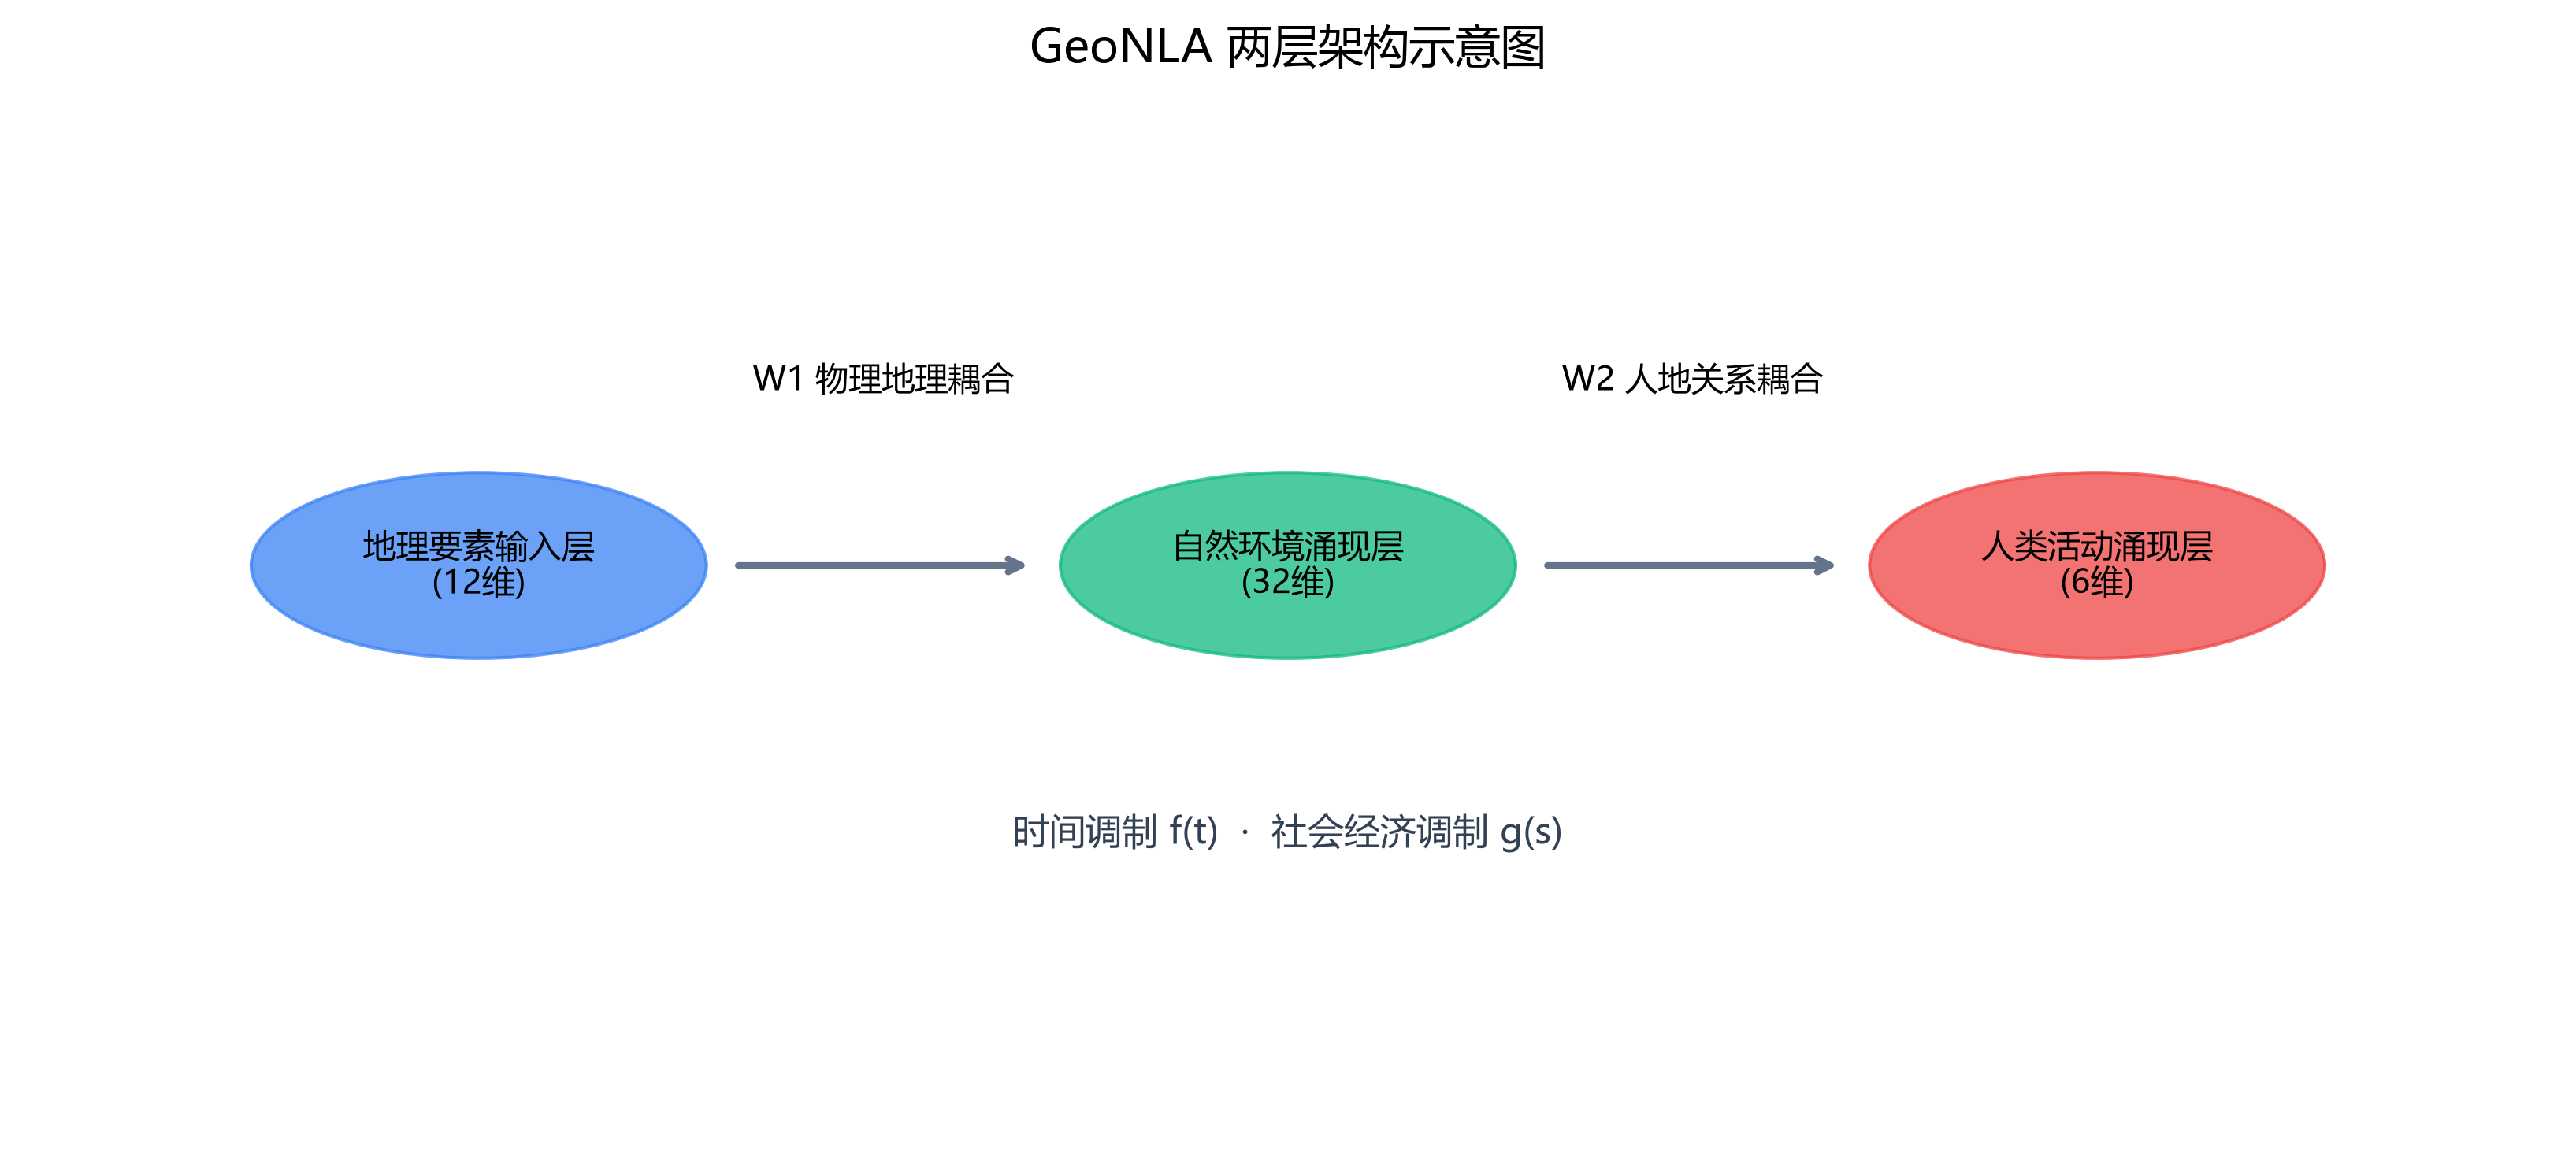
\includegraphics[width=0.85\textwidth]{../figures/fig1_model_architecture.png}
\caption{两层GeoNLA模型架构。物理层将12维地理输入变换为32维涌现表示，随后进行乘性时间调制，人类层将其映射到6维输出并附加社会经济调制。}
\label{fig:model_architecture}
\end{figure}

\subsection{FlatMLP基线}
\label{subsec:flatmlp}

基线模型移除了所有GeoNLA假设特有的结构归纳偏置：

\begin{itemize}
    \item \textbf{输入拼接：}地理特征（12维）、时间因子和社会经济因子拼接为单一14维输入向量。
    \item \textbf{两层MLP：} $\text{Linear}(14 \to 32) + \text{ReLU} + \text{Dropout}(0.2) \to \text{Linear}(32 \to 6) + \text{Sigmoid}$
    \item \textbf{无圈层涌现}，无乘性时间或社会经济调制。
\end{itemize}

\textbf{总可训练参数量：} 678。

参数量紧密匹配（652对678），确保任何性能差异反映的是架构归纳偏置而非模型容量。

%=============================================================
\section{实验设置}
\label{sec:experimental_setup}

所有实验均在PyTorch（$\geq$ 2.0）中实现，配置如下：

\begin{table}[htbp]
\centering
\caption{超参数配置。}
\label{tab:hyperparameters}
\begin{tabular}{ll}
\toprule
超参数 & 值 \\
\midrule
优化器 & Adam \\
学习率 & $1 \times 10^{-3}$ \\
权重衰减 & $1 \times 10^{-4}$ \\
学习率调度器 & ReduceLROnPlateau (patience=15, factor=0.5) \\
损失函数 & MSE \\
训练轮数 & 200 \\
批次大小 & 32 \\
随机种子 & 42 \\
\bottomrule
\end{tabular}
\end{table}

\textbf{评估指标。}我们报告在验证集上计算的三个指标：

\begin{itemize}
    \item \textbf{RMSE}（均方根误差）：度量整体预测量值误差。
    \item \textbf{MAE}（平均绝对误差）：度量平均绝对偏差。
    \item \textbf{R\textsuperscript{2}}（决定系数）：度量解释方差比例，报告所有输出维度的均值及每个单独输出维度的值。
\end{itemize}

\textbf{可复现性。}所有随机种子（Python、NumPy、PyTorch CPU/CUDA）均固定为42。代码库、数据生成脚本和训练模型检查点与本报告一同归档。

%=============================================================
\section{结果}
\label{sec:results}

\subsection{合成数据实验}
\label{subsec:synthetic_results}

表~\ref{tab:synthetic_overall}总结了合成数据上的整体验证性能。

\begin{table}[htbp]
\centering
\caption{合成数据上的整体验证指标（400样本，80/20划分）。}
\label{tab:synthetic_overall}
\begin{tabular}{lcccc}
\toprule
模型 & 参数量 & RMSE $\downarrow$ & MAE $\downarrow$ & $R^2$（均值）$\uparrow$ \\
\midrule
GeoNLA & 652 & 0.1140 & 0.0790 & 0.7918 \\
FlatMLP & 678 & 0.1221 & 0.0912 & 0.7621 \\
\textbf{改进} & --- & \textbf{$-6.6\%$} & \textbf{$-13.3\%$} & \textbf{$+0.030$} \\
\bottomrule
\end{tabular}
\end{table}

GeoNLA在三个指标上均实现了显著提升。最显著的增益出现在MAE（$-13.3\%$），表明具有乘性调制的分层架构比平坦基线更有效地减少了大预测误差。

表~\ref{tab:synthetic_perdim}给出了逐维 $R^2$ 分解，揭示了架构优势最为集中的位置。

\begin{table}[htbp]
\centering
\caption{合成数据上的逐维 $R^2$。}
\label{tab:synthetic_perdim}
\begin{tabular}{lccc}
\toprule
输出维度 & GeoNLA & FlatMLP & $\Delta$ \\
\midrule
耕地比例 & 0.710 & 0.651 & $+0.059$ \\
灌溉比例 & 0.822 & 0.746 & $+0.076$ \\
建设用地 & 0.711 & 0.700 & $+0.011$ \\
人口密度 & 0.891 & 0.880 & $+0.011$ \\
夜间灯光 & 0.829 & 0.838 & $-0.009$ \\
道路密度 & 0.787 & 0.757 & $+0.030$ \\
\bottomrule
\end{tabular}
\end{table}

最大改进出现在\textbf{灌溉比例}（$+0.076$）和\textbf{耕地比例}（$+0.059$），这两者均受到物理地理级联（地形 $\to$ 气候 $\to$ 土壤 $\to$ 水资源可利用性）的强烈控制。这与GeoNLA假设一致：这些输出从分层地理变换中获益最多。夜间灯光呈现边际下降（$-0.009$），可能是因为其与物理地理的关系更为直接，较少通过圈层叠加级联中介。

\begin{figure}[htbp]
\centering
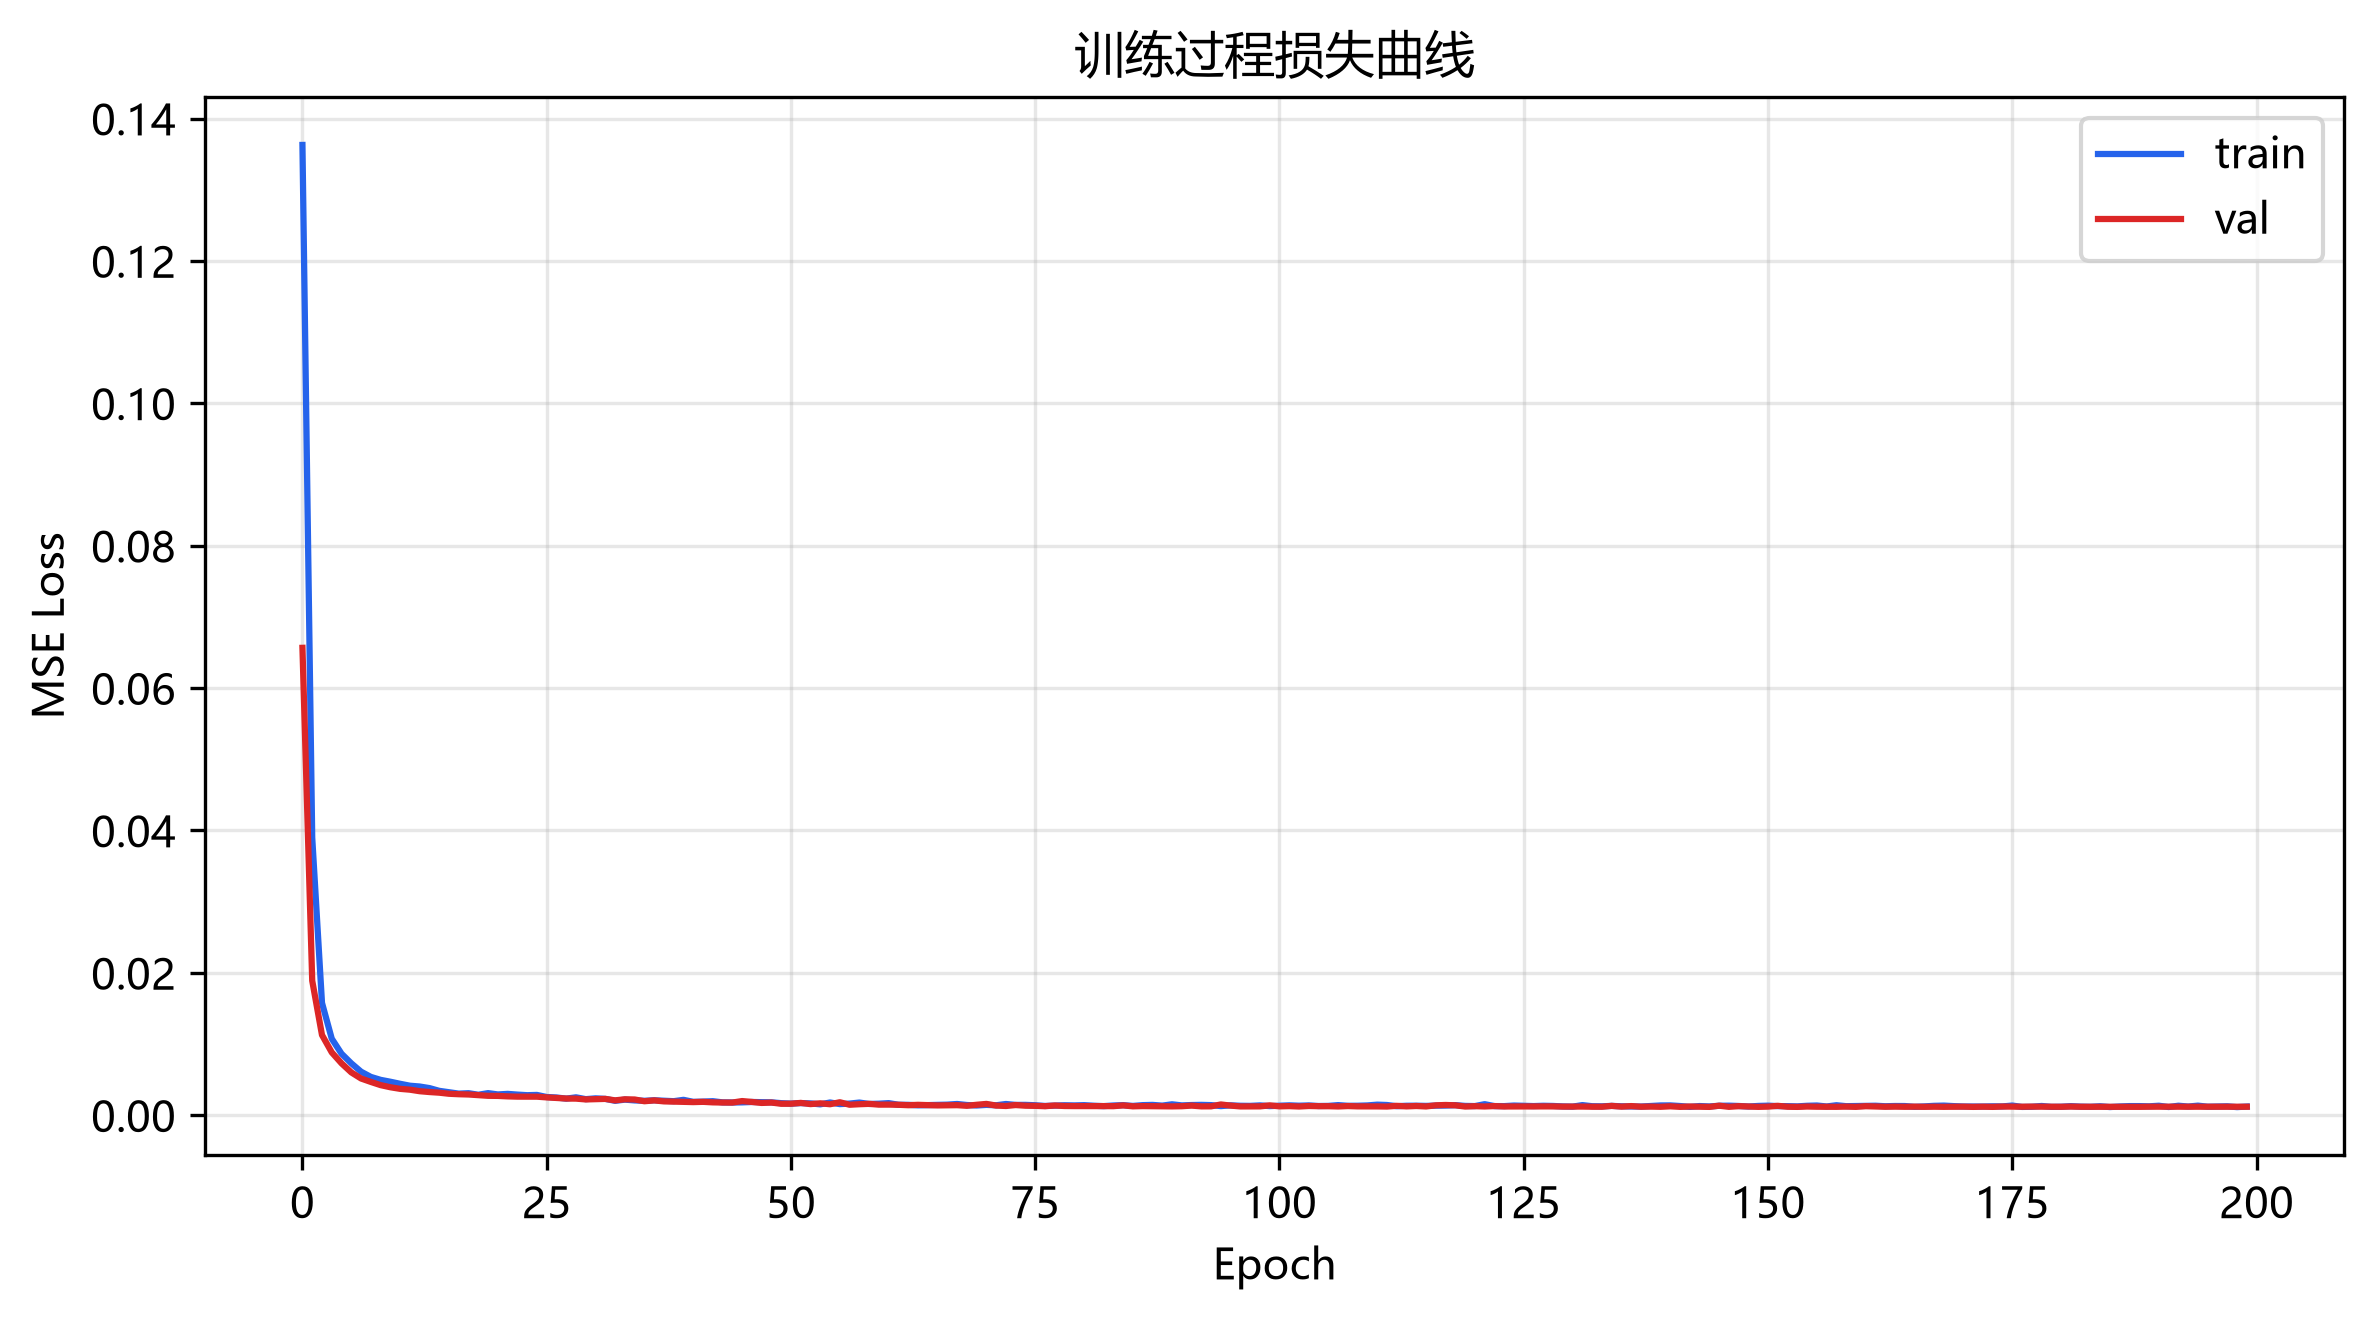
\includegraphics[width=\textwidth]{../figures/fig0_loss_curves.png}
\caption{GeoNLA与FlatMLP在合成数据上的训练和验证损失曲线。}
\label{fig:loss_curves}
\end{figure}

\begin{figure}[htbp]
\centering
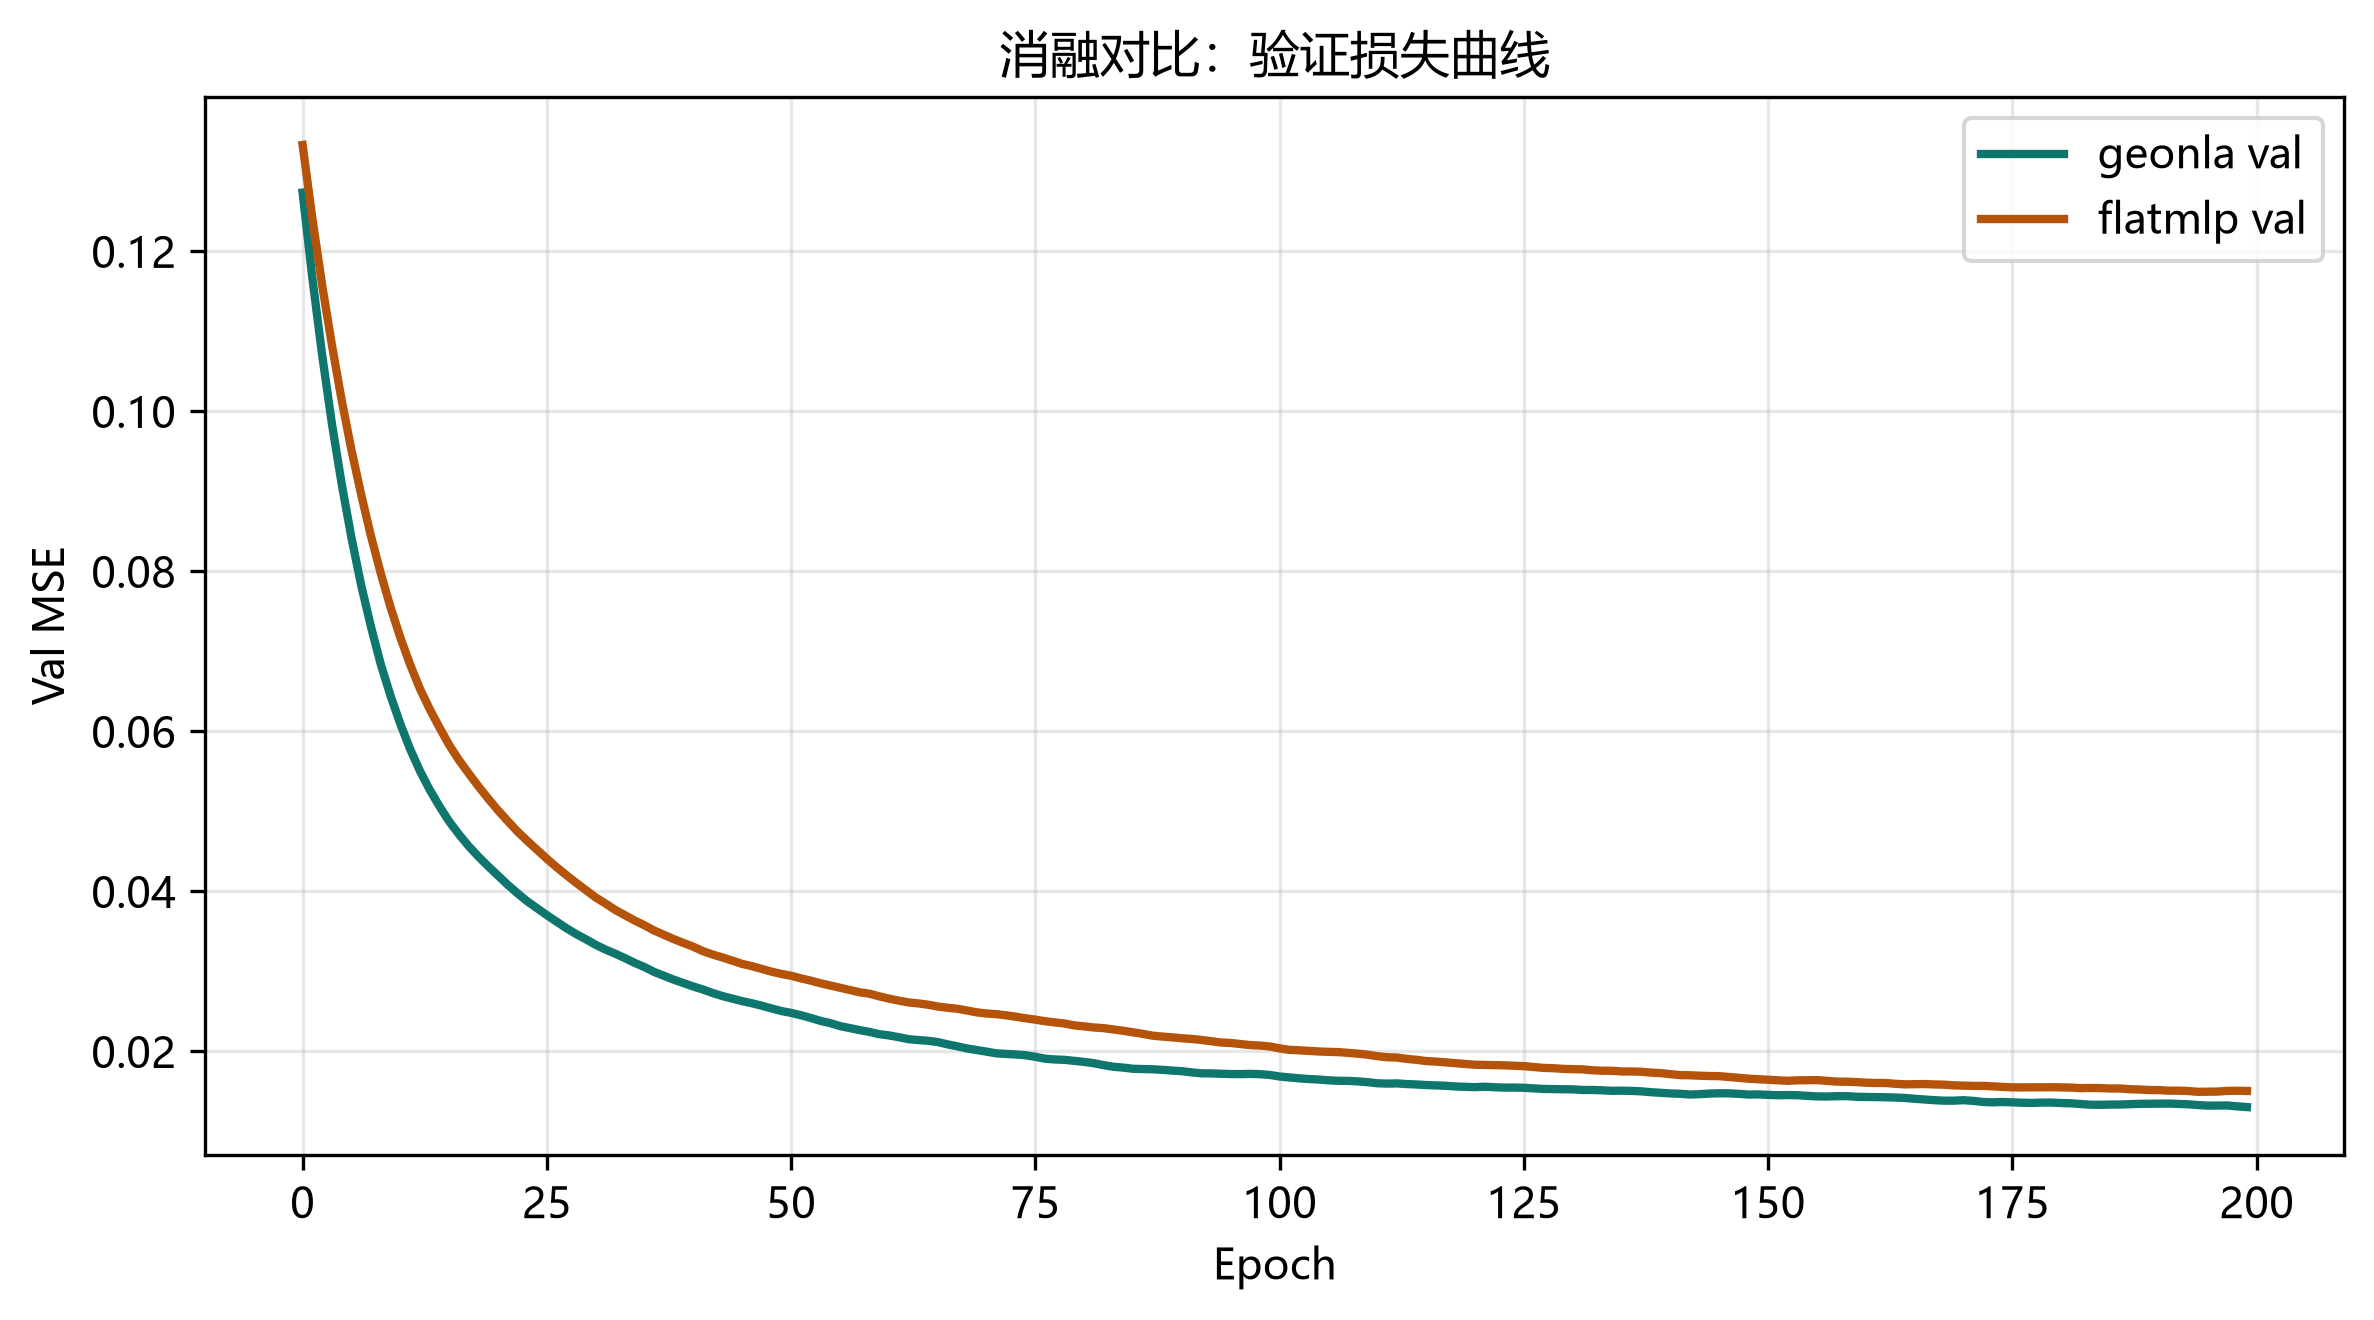
\includegraphics[width=0.75\textwidth]{../figures/fig6_ablation_val_loss.png}
\caption{验证损失比较：GeoNLA vs.\ FlatMLP。}
\label{fig:ablation_val_loss}
\end{figure}

\begin{figure}[htbp]
\centering
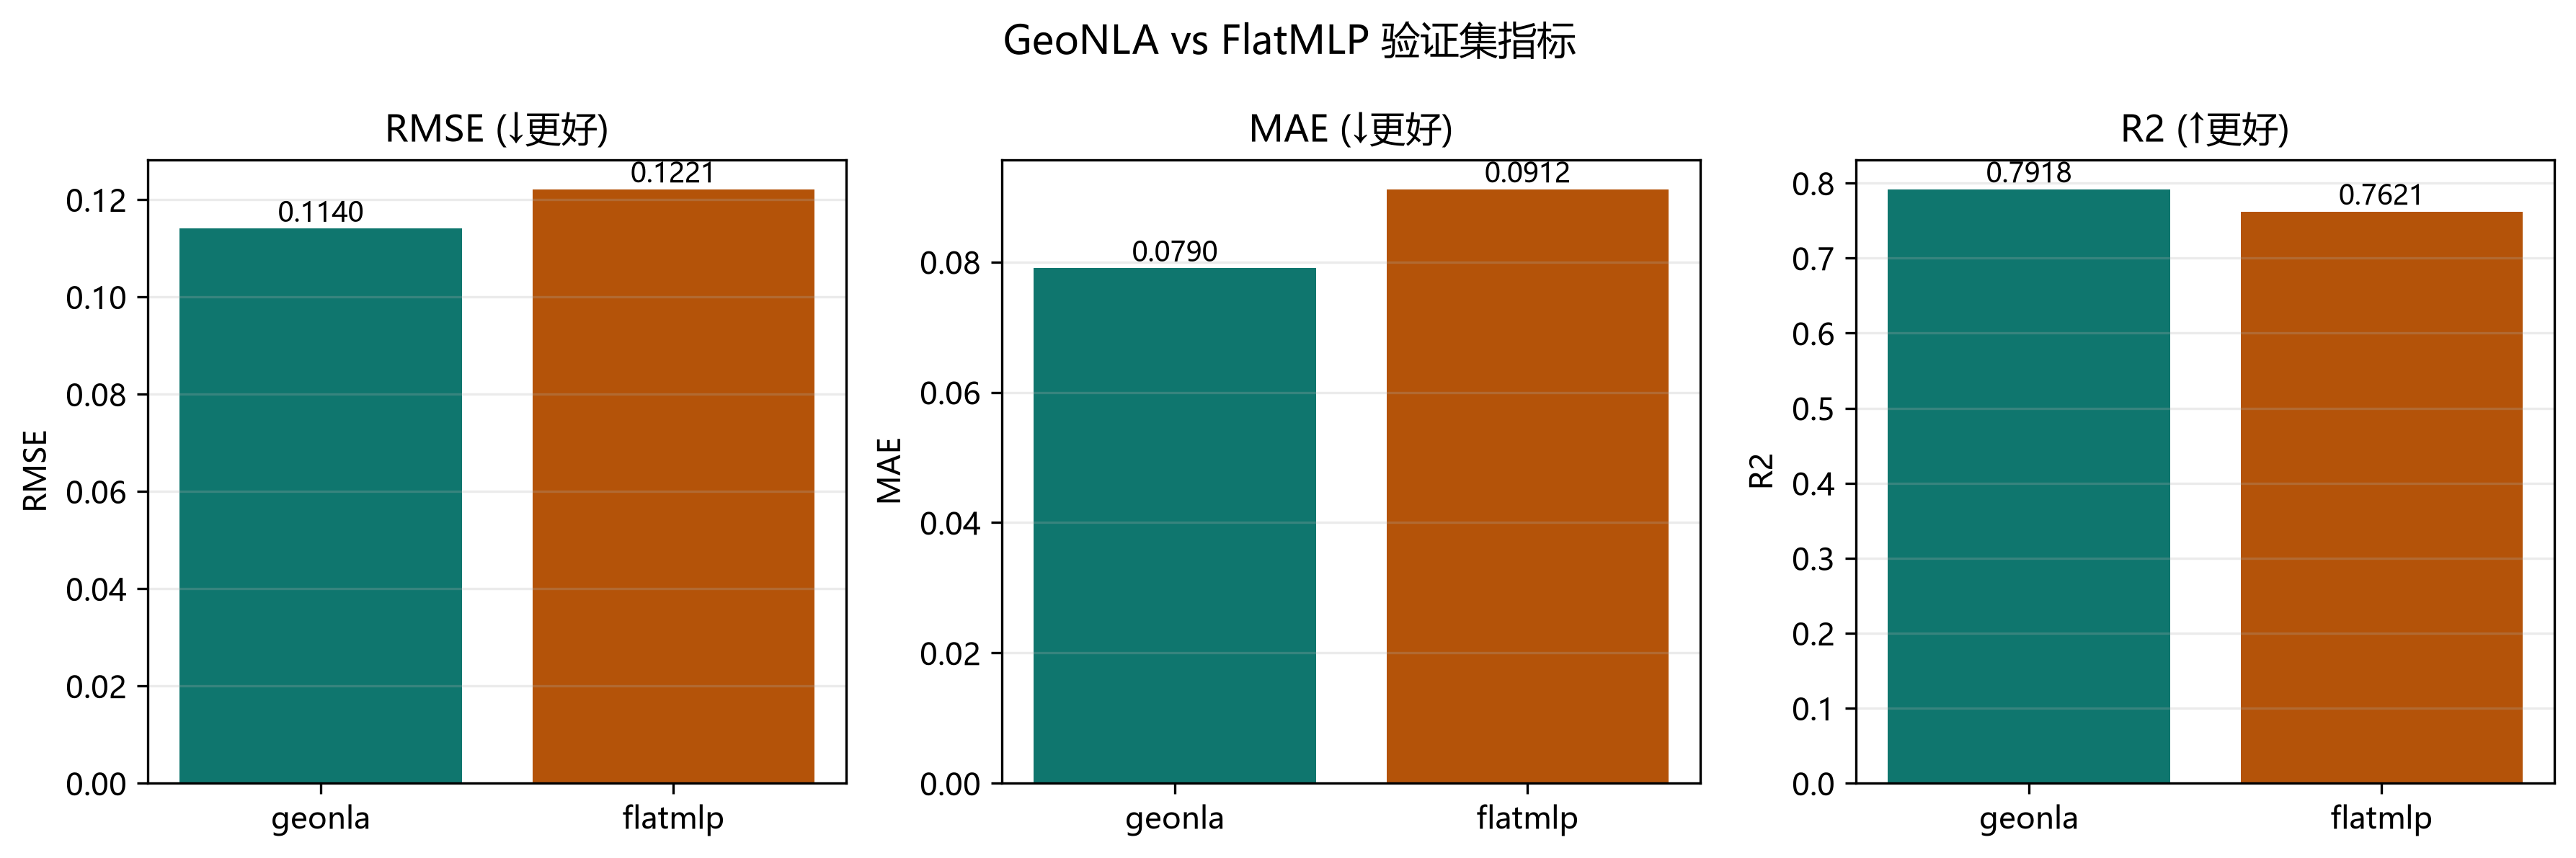
\includegraphics[width=\textwidth]{../figures/fig7_ablation_metrics.png}
\caption{GeoNLA与FlatMLP的RMSE、MAE和 $R^2$ 比较柱状图。}
\label{fig:ablation_metrics}
\end{figure}

\begin{figure}[htbp]
\centering
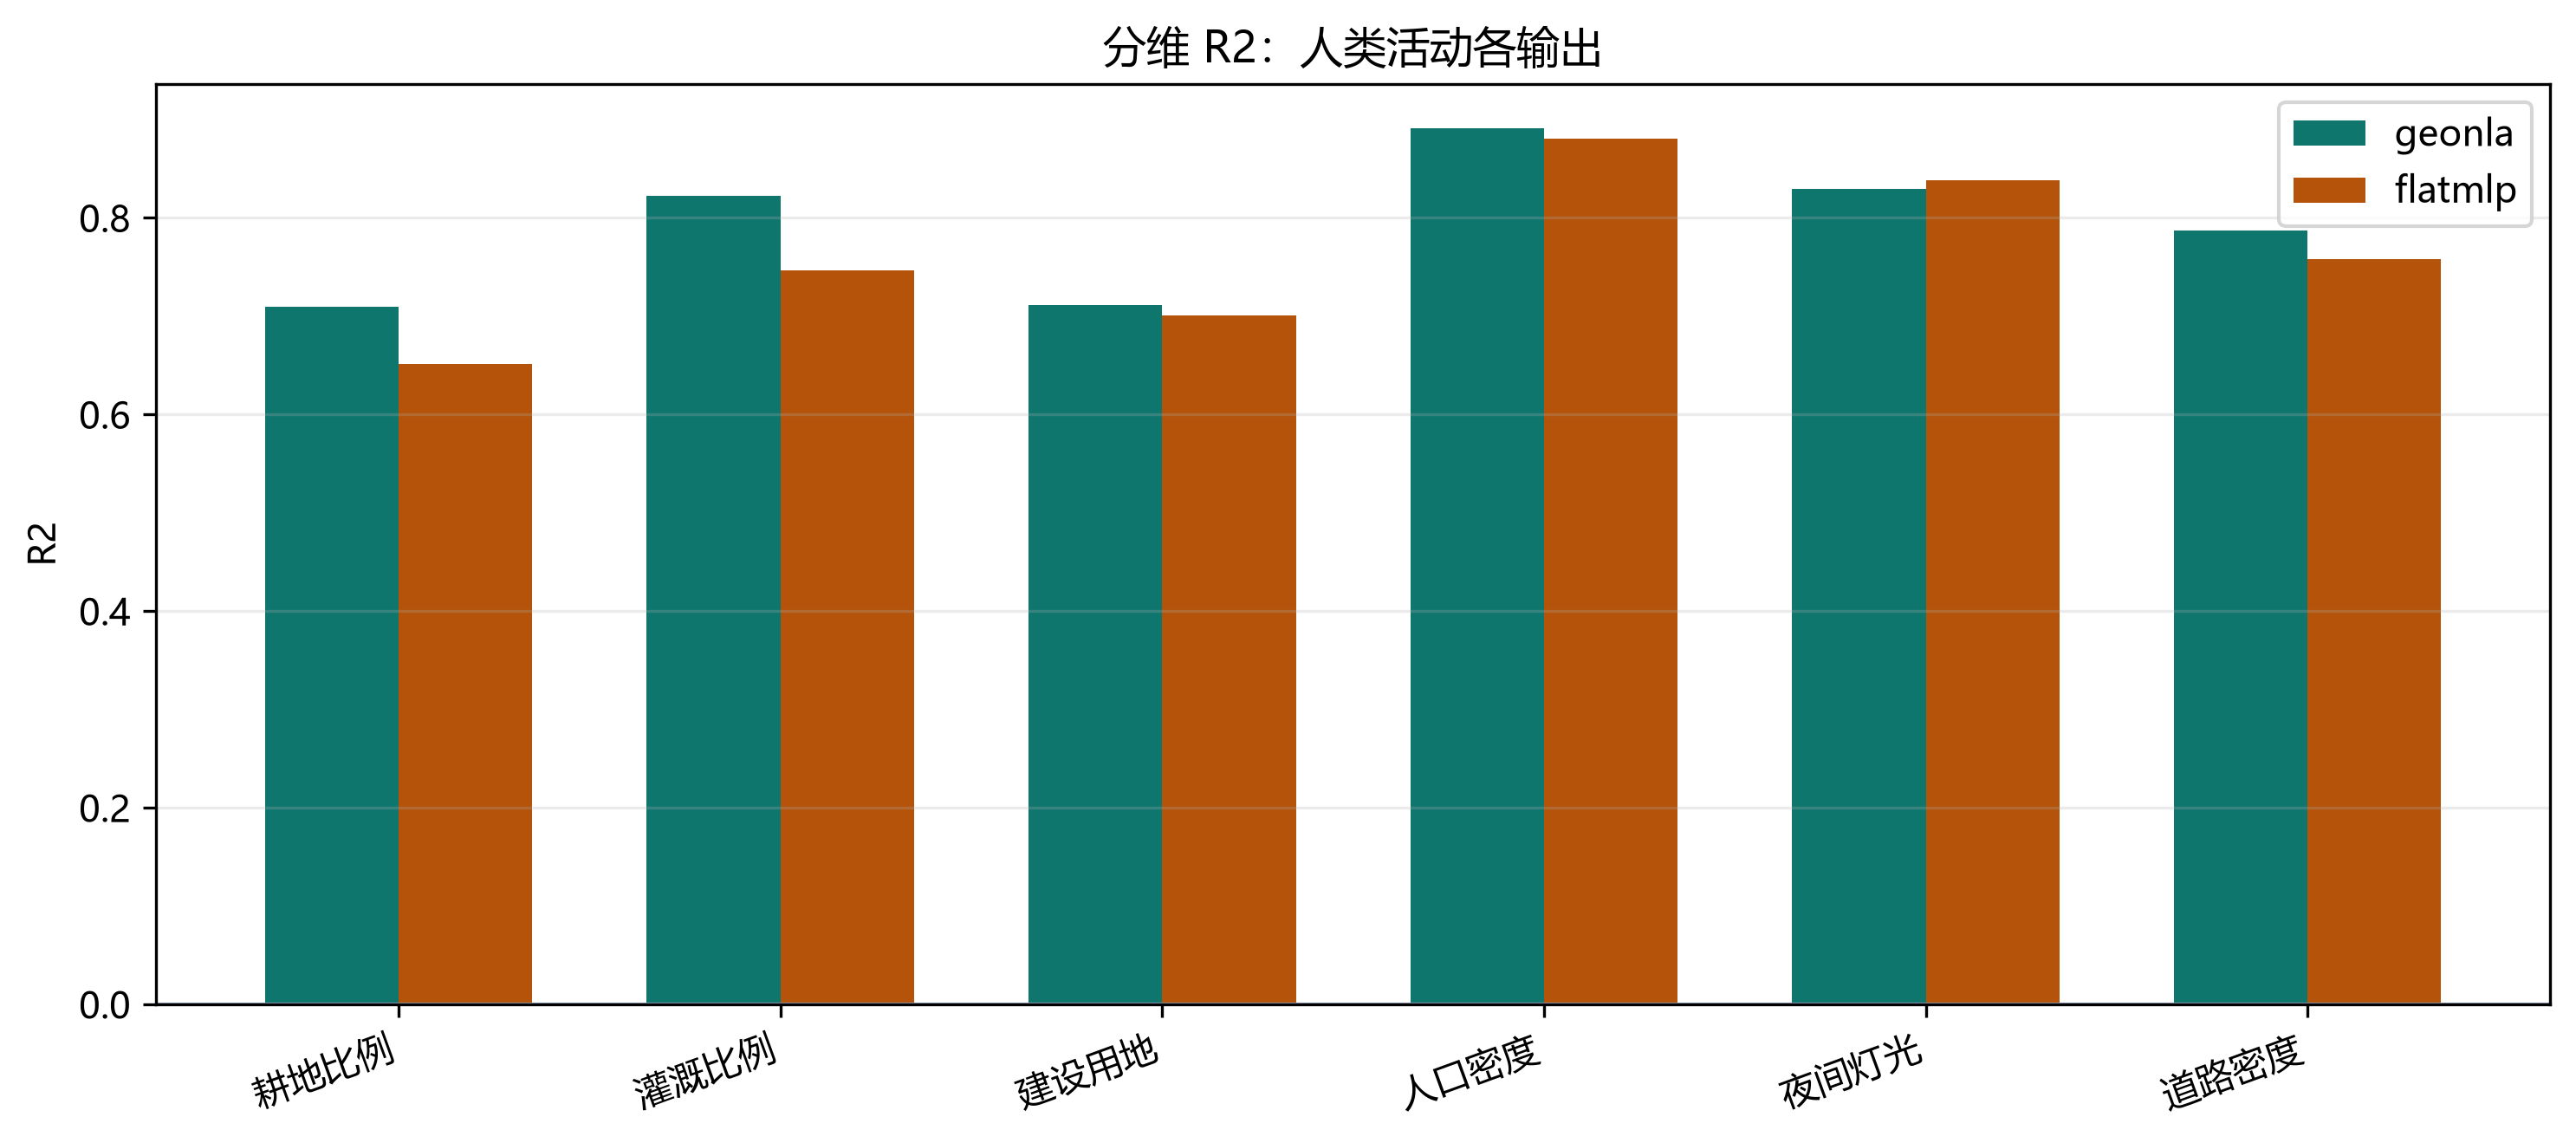
\includegraphics[width=\textwidth]{../figures/fig8_ablation_r2_per_dim.png}
\caption{合成数据上GeoNLA与FlatMLP的逐维 $R^2$ 比较。}
\label{fig:ablation_r2_per_dim}
\end{figure}

\subsection{真实栅格数据实验}
\label{subsec:real_results}

表~\ref{tab:real_overall}展示了临夏盆地真实栅格数据集上的结果。

\begin{table}[htbp]
\centering
\caption{真实栅格数据上的整体验证指标（临夏盆地，${\sim}1$\,km网格）。}
\label{tab:real_overall}
\begin{tabular}{lcccc}
\toprule
模型 & 参数量 & RMSE $\downarrow$ & MAE $\downarrow$ & $R^2$（均值）$\uparrow$ \\
\midrule
GeoNLA & 652 & 0.0342 & 0.0114 & 0.9120 \\
FlatMLP & 678 & 0.0351 & 0.0117 & 0.9107 \\
\textbf{改进} & --- & \textbf{$-2.7\%$} & \textbf{$-3.1\%$} & \textbf{$+0.001$} \\
\bottomrule
\end{tabular}
\end{table}

改进方向一致，但与合成实验相比幅度较小。两个模型均达到较高的 $R^2$ 值（$\geq 0.91$），反映了${\sim}1$\,km网格化真实数据中相对平滑的关系。

\begin{table}[htbp]
\centering
\caption{真实栅格数据上的逐维 $R^2$。}
\label{tab:real_perdim}
\begin{tabular}{lccc}
\toprule
输出维度 & GeoNLA & FlatMLP & $\Delta$ \\
\midrule
建设用地 & 0.850 & 0.837 & $+0.013$ \\
人口密度 & 0.955 & 0.958 & $-0.003$ \\
夜间灯光 & 0.971 & 0.976 & $-0.005$ \\
道路密度 & 0.872 & 0.872 & $0.000$ \\
\bottomrule
\end{tabular}
\end{table}

GeoNLA在\textbf{建设用地}上展现了最大优势（$+0.013$），该输出整合了多种物理地理约束（地形适宜性、水资源获取、土地覆被）。对于人口密度和夜间灯光——具有更直接统计关系的变量——两个模型表现相当。道路密度显示完全相同的性能，表明架构差异对该特定输出的影响极小。

\begin{figure}[htbp]
\centering
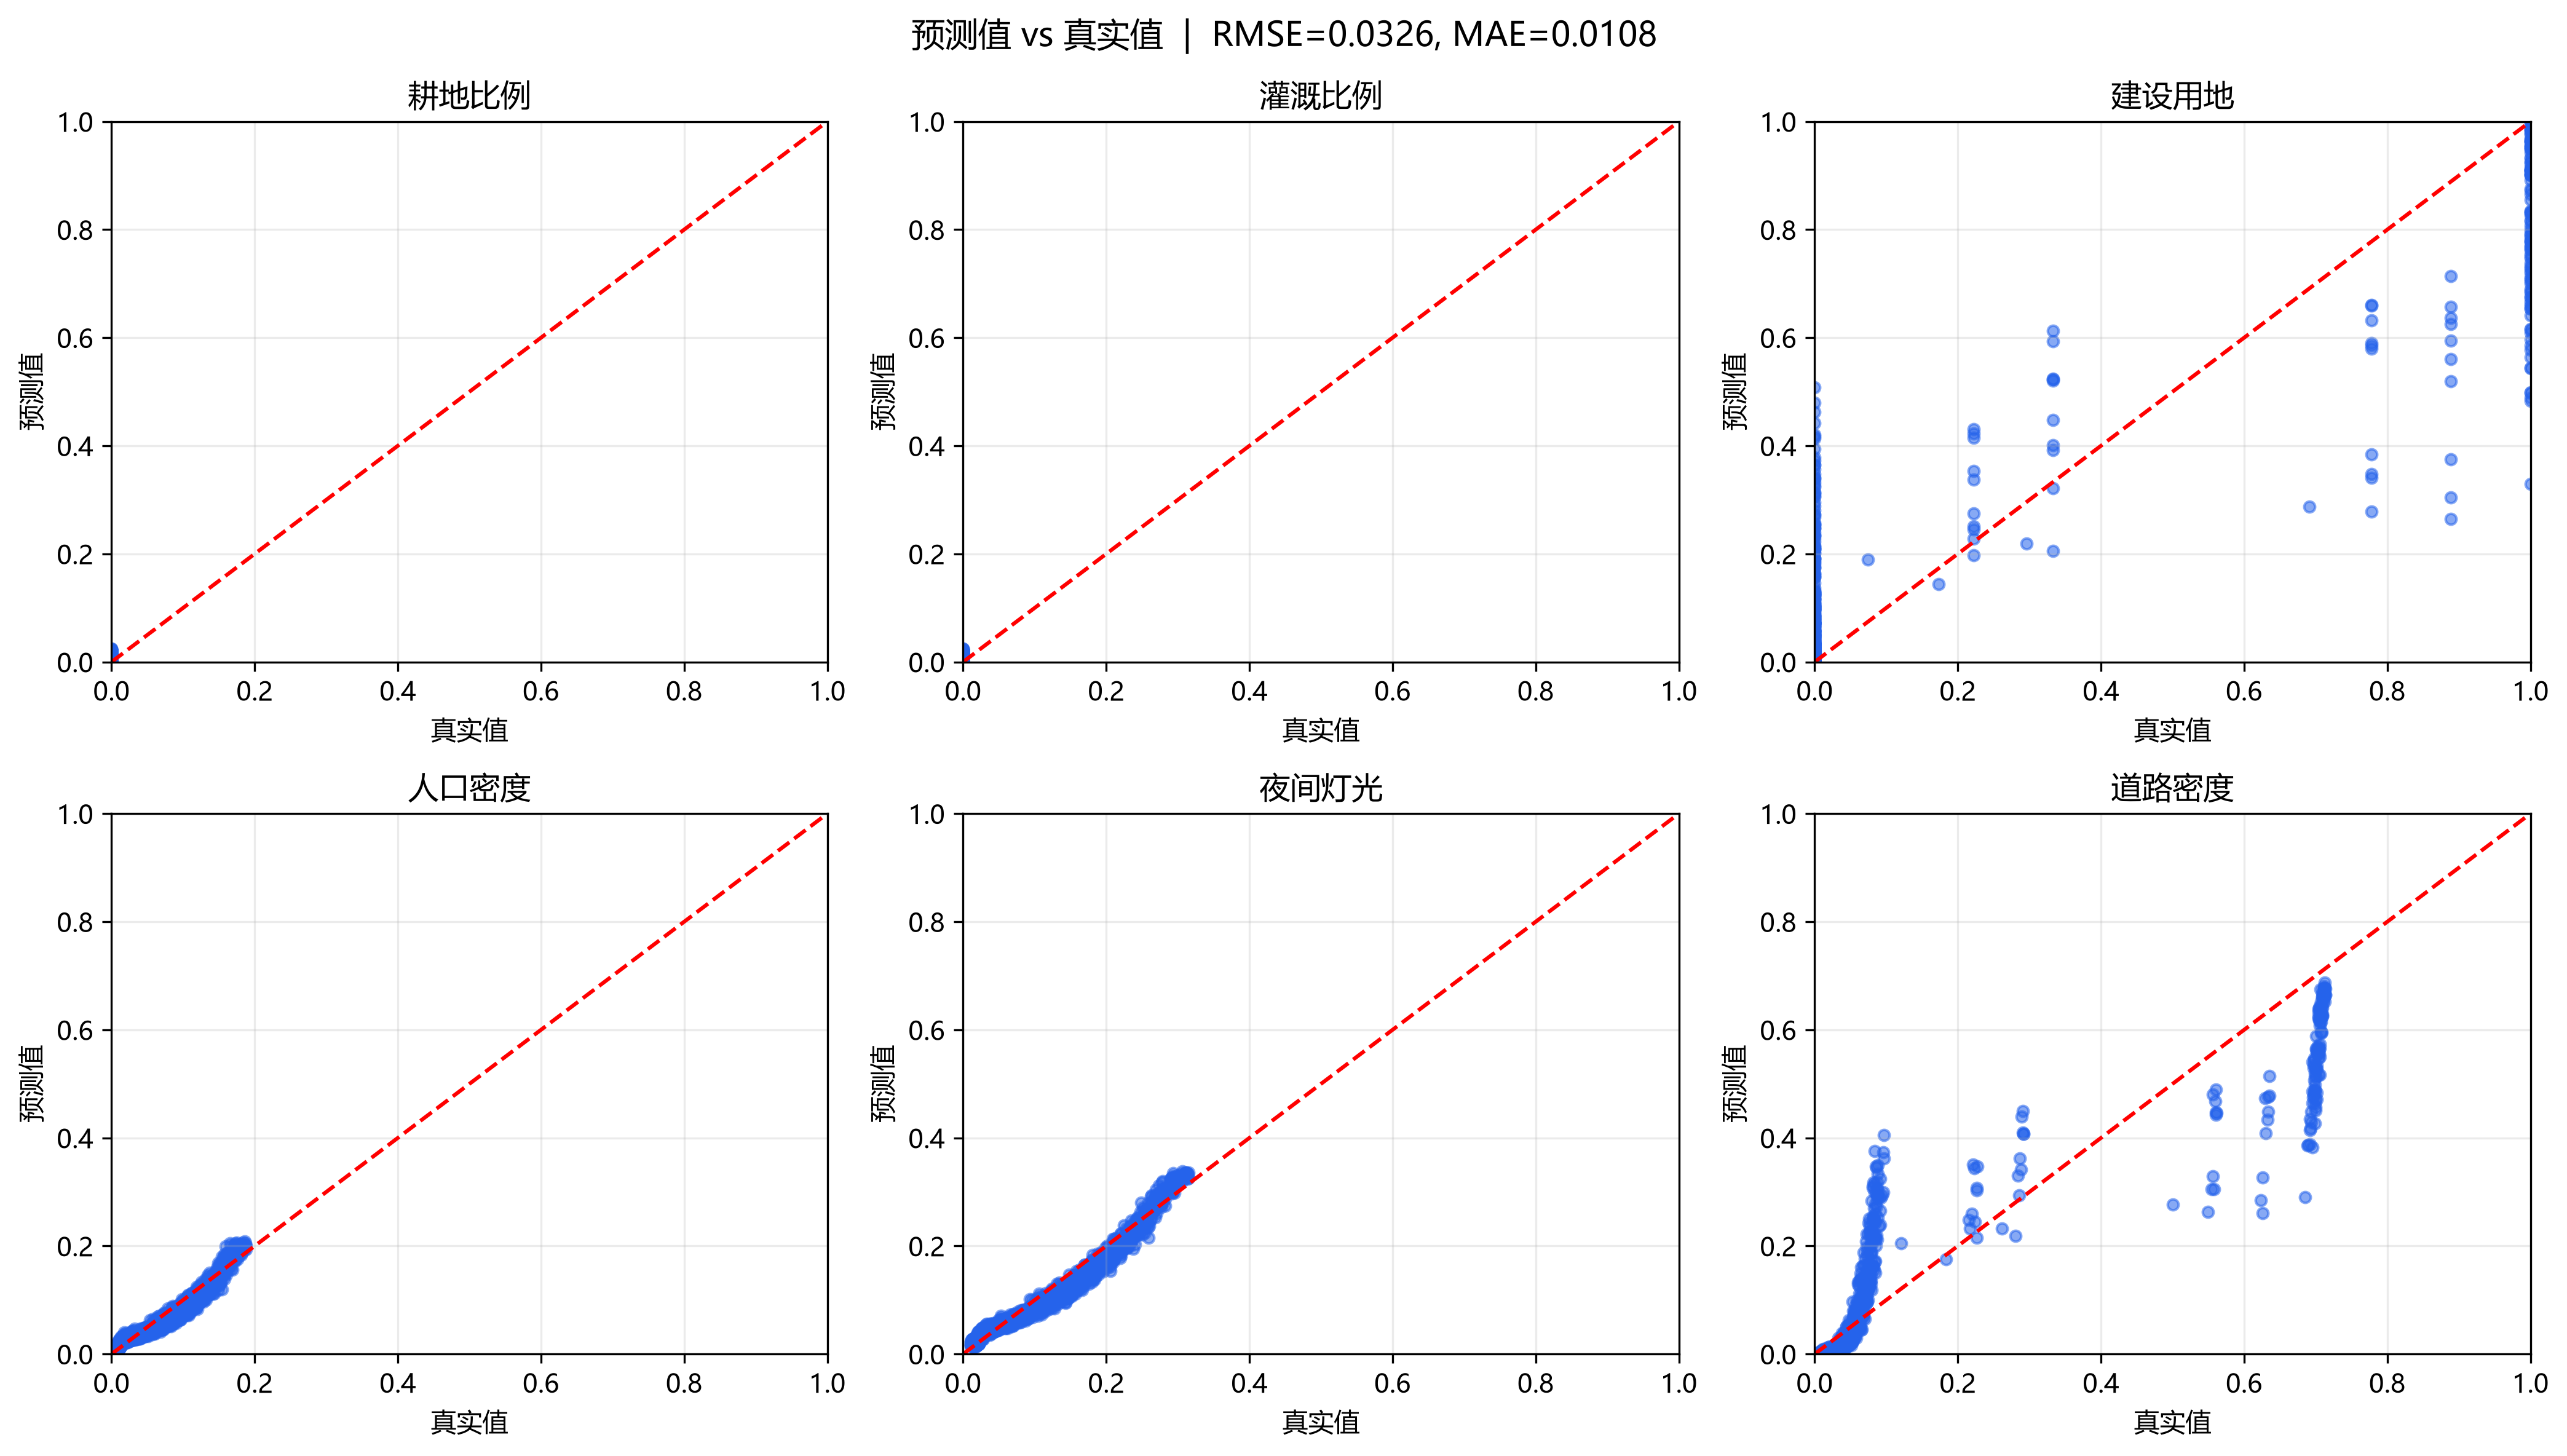
\includegraphics[width=\textwidth]{../figures/fig3_prediction_comparison.png}
\caption{真实栅格数据上所有输出维度的预测值 vs.\ 真实值散点图。}
\label{fig:prediction_comparison}
\end{figure}

\subsection{关键可视化}
\label{subsec:key_vis}

\textbf{涌现层的t-SNE分析。}32维涌现表示（阶段~1输出）的t-SNE投影揭示，GeoNLA保留了地理相似性结构：来自相似地形-气候-土壤簇的网格单元在嵌入空间中位置接近，而来自不同地理环境的单元则良好分离。

\begin{figure}[htbp]
\centering
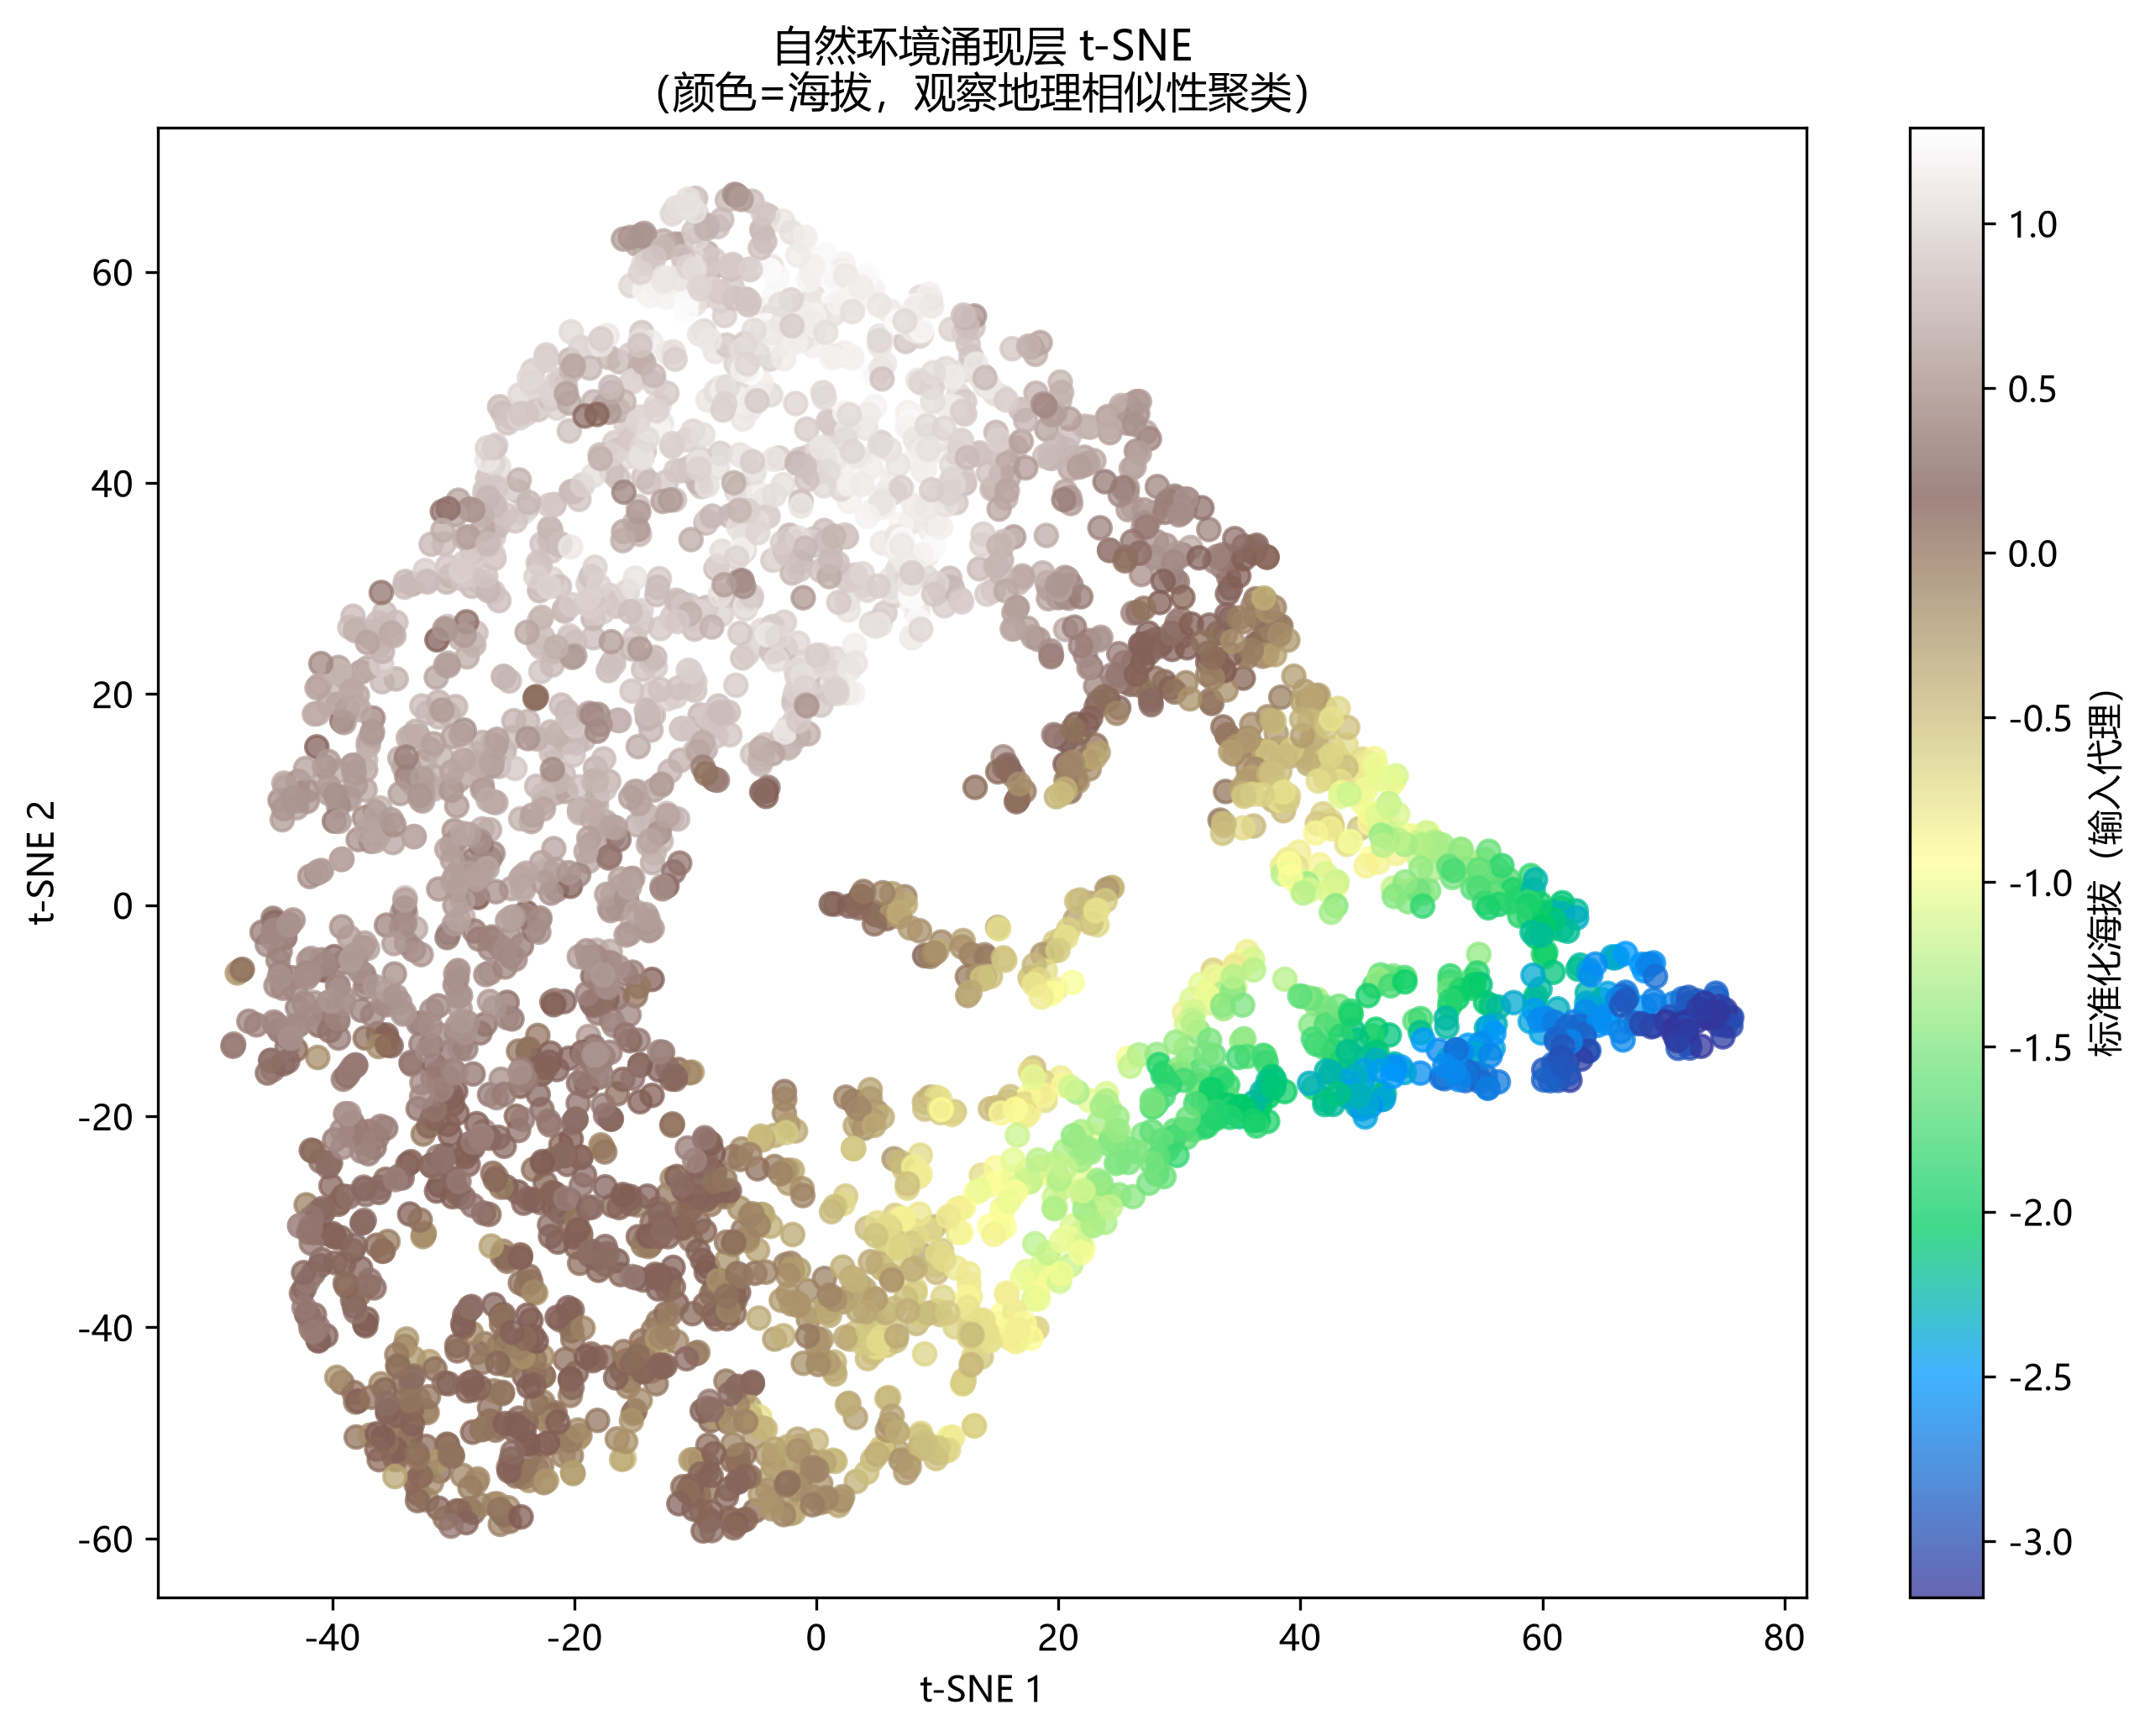
\includegraphics[width=\textwidth]{../figures/fig2_emergence_tsne.png}
\caption{32维涌现层的t-SNE可视化。GeoNLA保留了地理相似性结构，来自相似地形-气候-土壤簇的单元位置接近。}
\label{fig:emergence_tsne}
\end{figure}

\textbf{权重热力图。}学习得到的 $W_1$（物理耦合，$12 \times 32$）和 $W_2$（人地耦合，$32 \times 6$）权重矩阵揭示了可解释的耦合路径。$W_1$展示了与四个地理圈层对应的连贯块状结构，每个圈层对涌现表示贡献独特特征。$W_2$揭示了哪些涌现特征驱动哪些人类活动输出。

\begin{figure}[htbp]
\centering
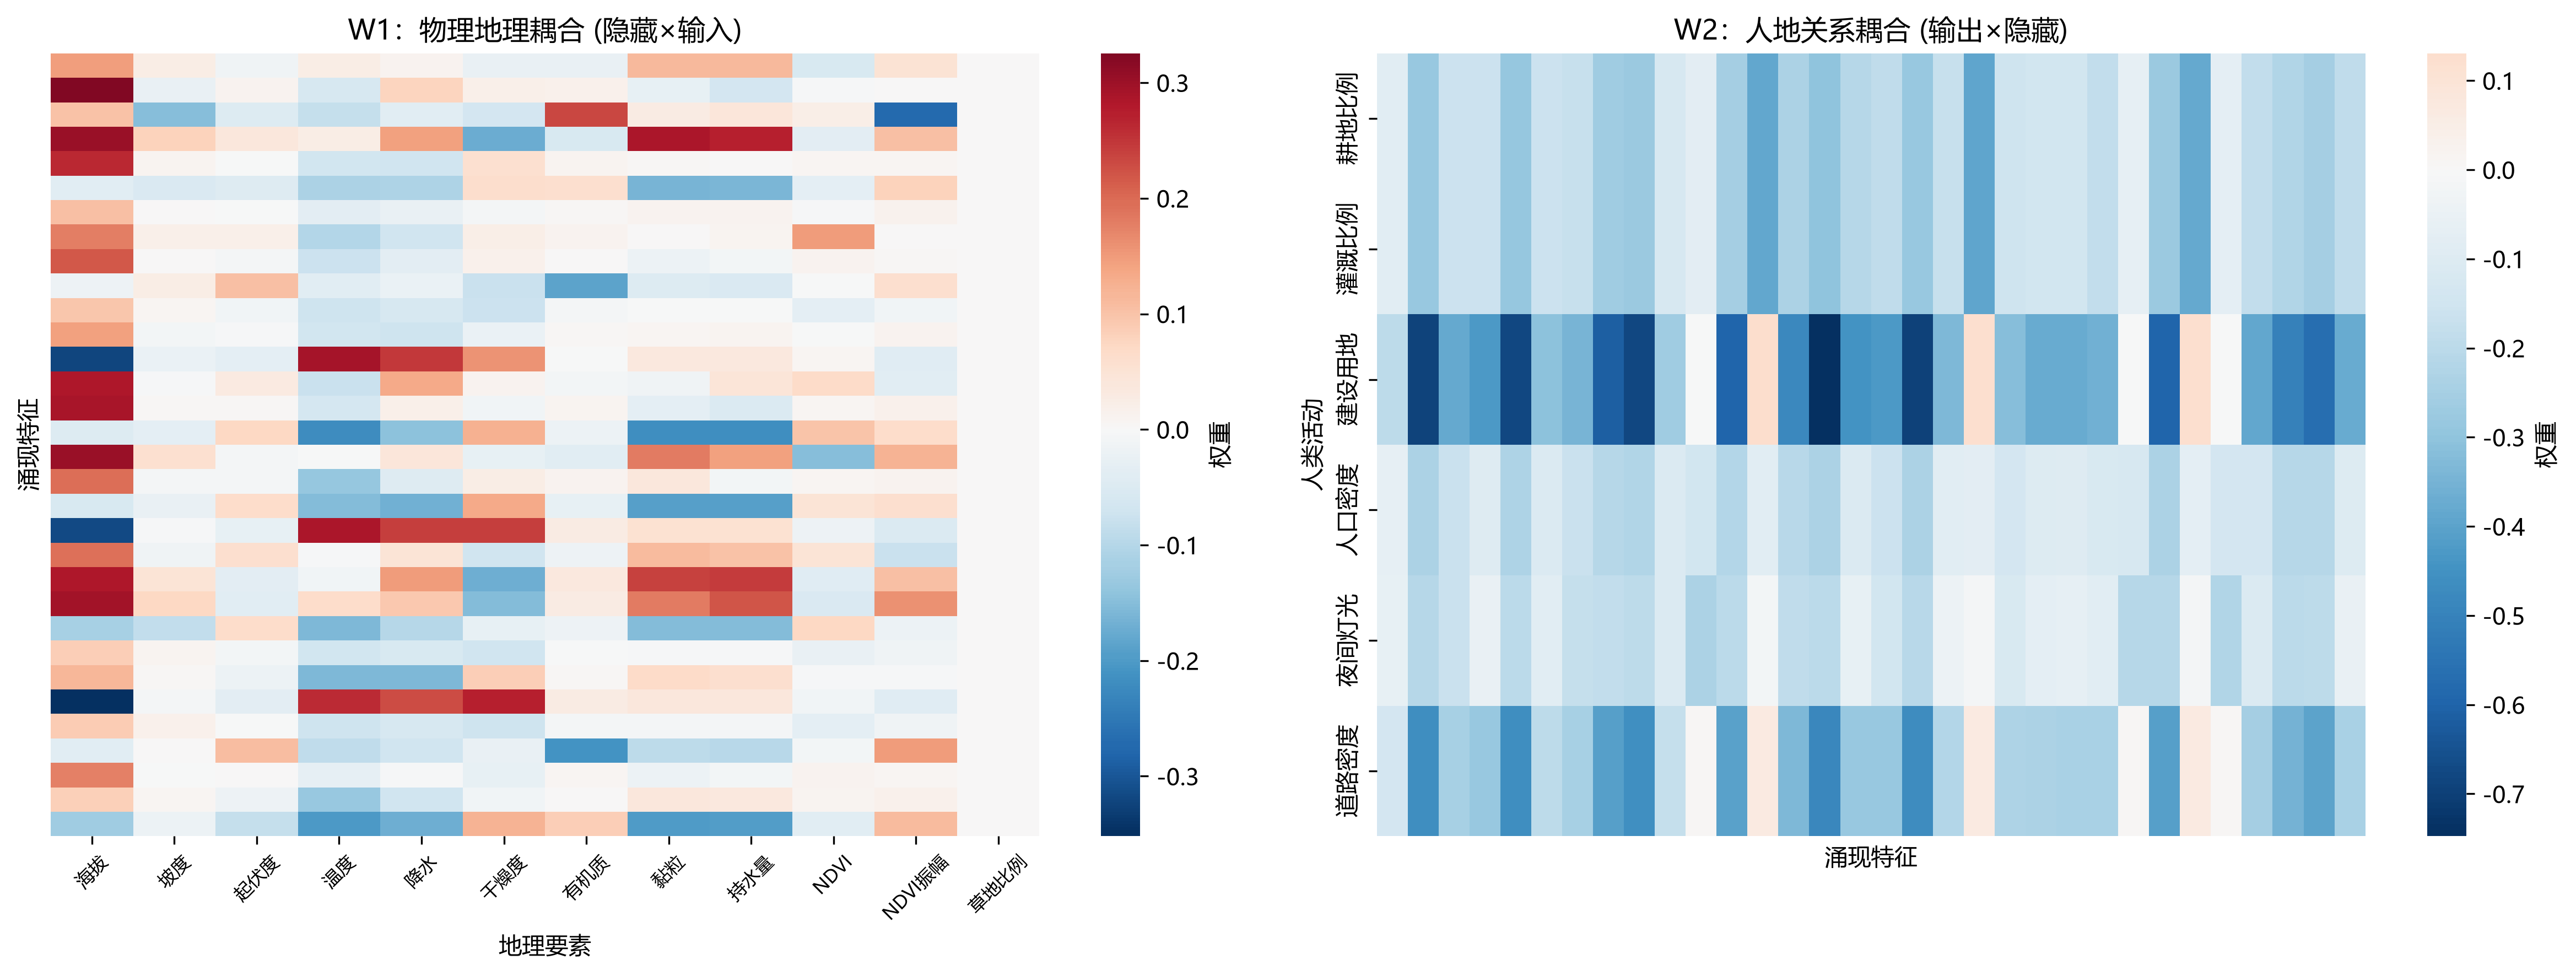
\includegraphics[width=\textwidth]{../figures/fig4_weight_heatmaps.png}
\caption{学习得到的权重热力图。上方：$W_1$（物理耦合，$12 \times 32$），展示与四个地理圈层对应的连贯块状结构。下方：$W_2$（人地耦合，$32 \times 6$），揭示哪些涌现特征驱动人类活动输出。}
\label{fig:weight_heatmaps}
\end{figure}

\textbf{时间调制效应。}时间调制可视化展示了固定地理条件下12个月的预测人类活动值。乘性调制产生了逼真的季节变化——农业输出在生长季达到峰值，而建筑和人口相关输出呈现不同的时间模式——验证了GeoNLA框架中乘性时间耦合机制的作用。

\begin{figure}[htbp]
\centering
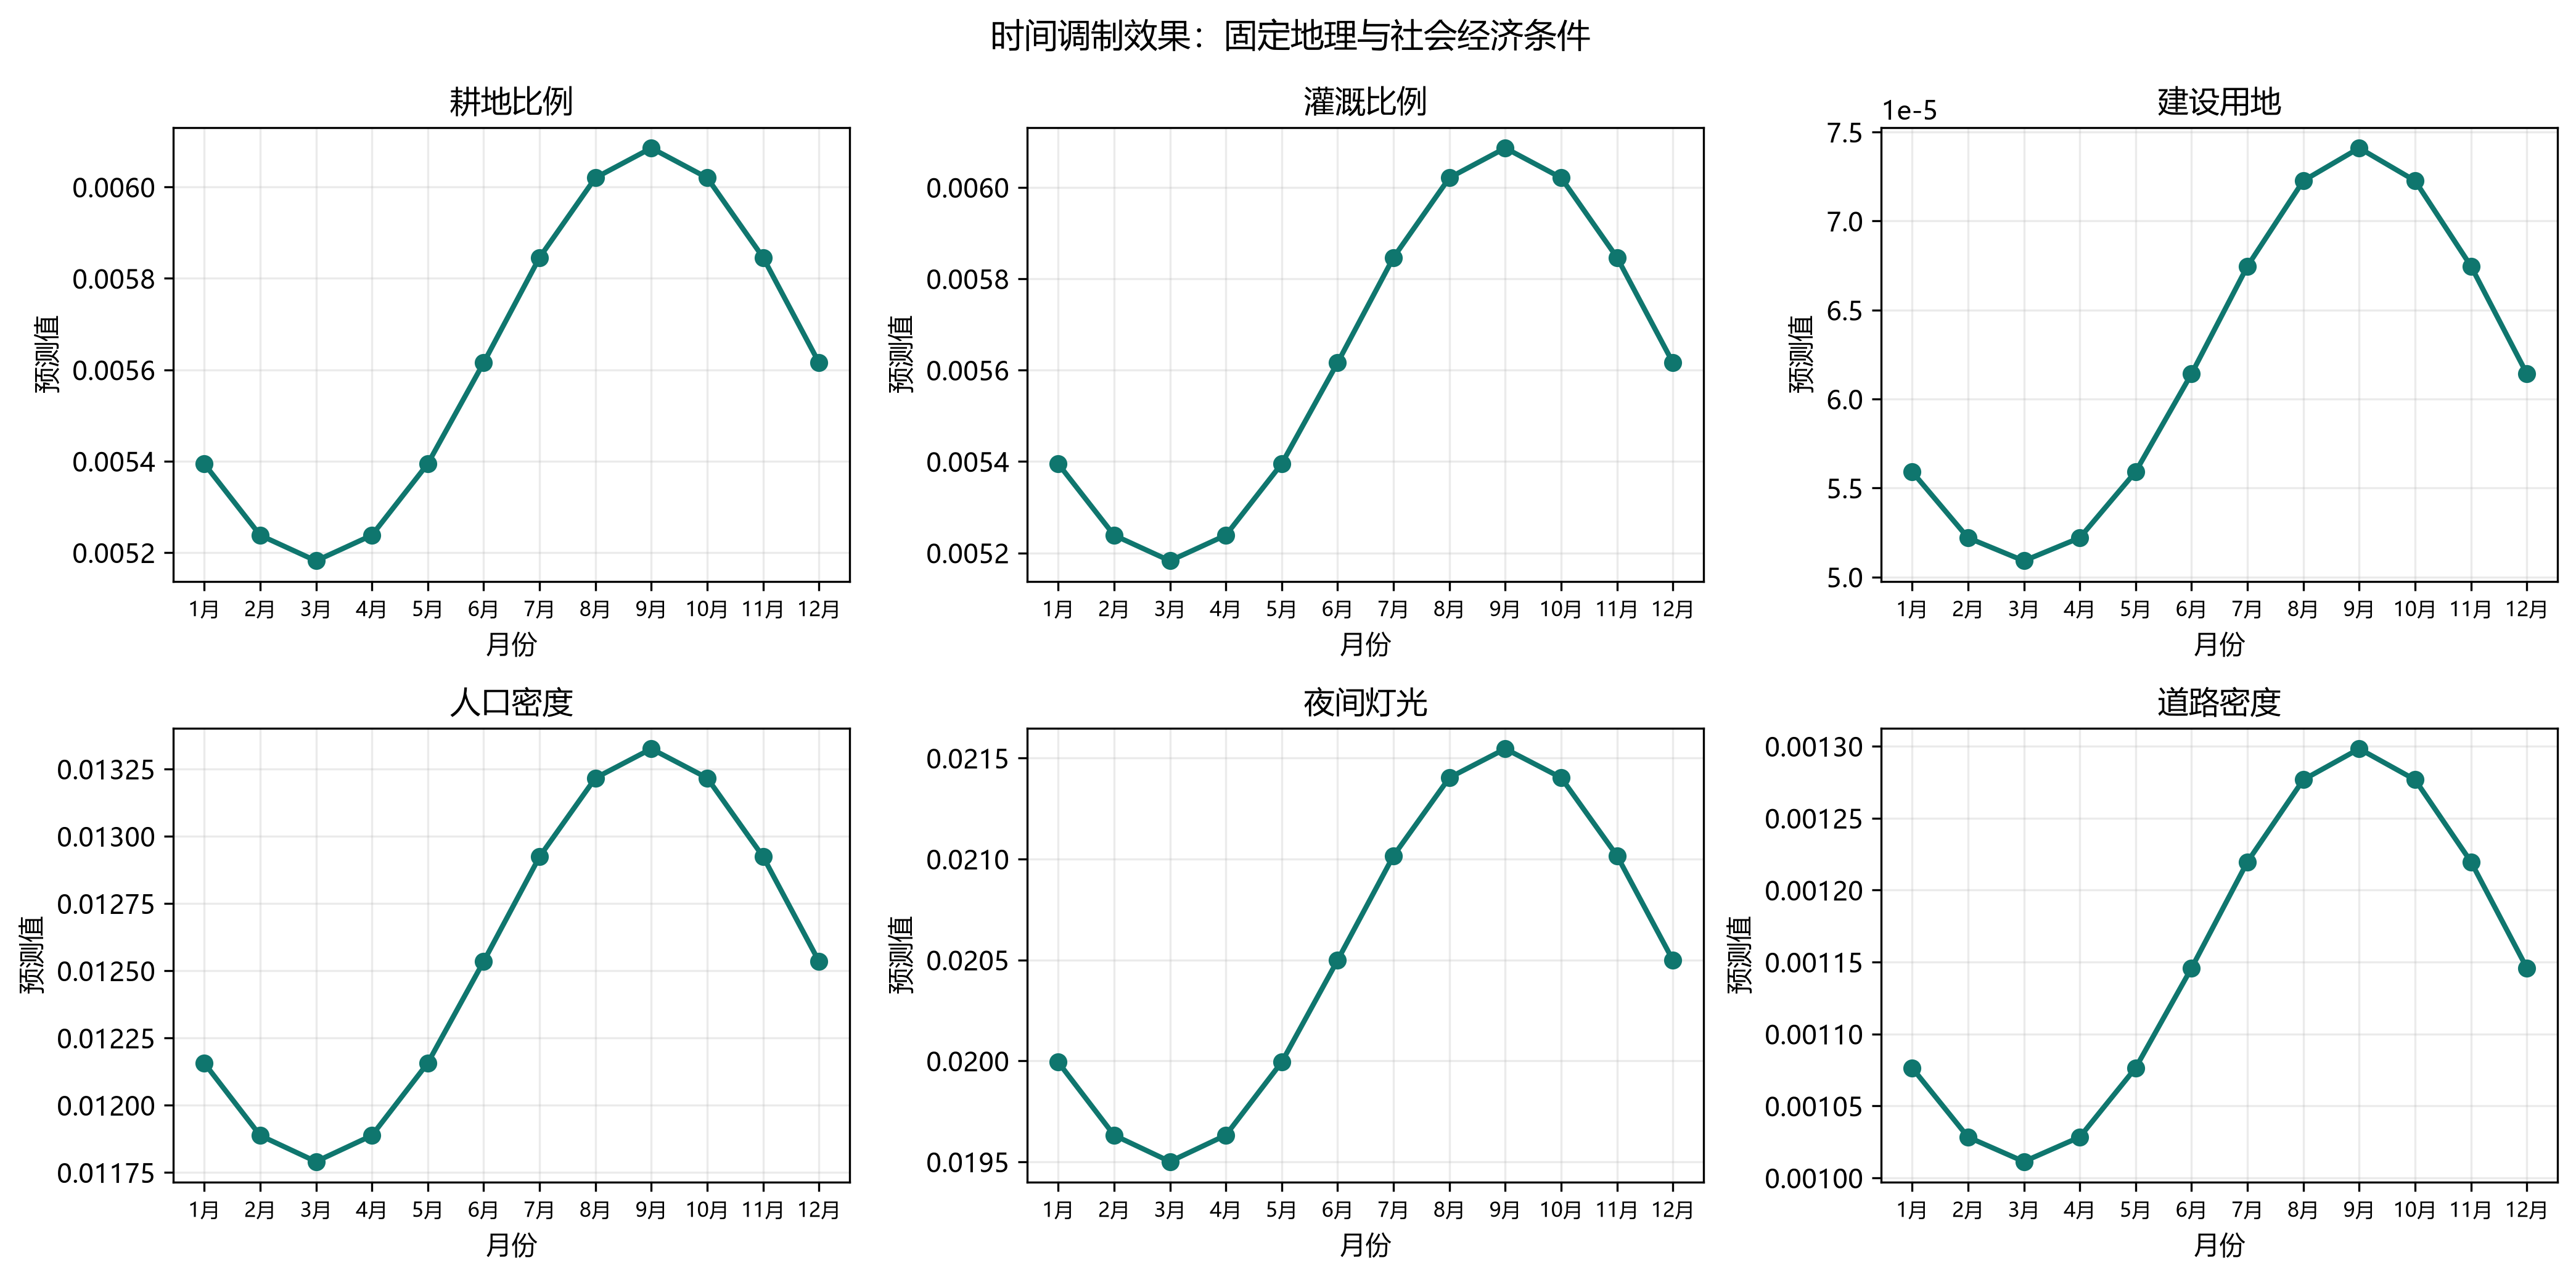
\includegraphics[width=\textwidth]{../figures/fig5_temporal_modulation.png}
\caption{12个月的时间调制效应。固定地理条件下的预测人类活动值显示了由乘性时间耦合驱动的真实现实季节变化。}
\label{fig:temporal_modulation}
\end{figure}

%=============================================================
\section{讨论}
\label{sec:discussion}

\subsection{架构归纳偏置}
\label{subsec:inductive_bias}

实验结果一致支持核心GeoNLA假设：具有乘性调制的分层架构在建模地理人地关系方面优于参数匹配的平坦MLP。在合成数据上——数据生成过程精确对应GeoNLA公式——优势显著——RMSE降低6.6\%，MAE降低13.3\%。在真实栅格数据上，优势持续但减弱（RMSE降低2.7\%），这是预期之中的，因为真实世界标签由遥感产品派生而非由严格的两层乘性过程生成。

参数匹配设计（652对678个参数）至关重要：性能增益不能归因于模型容量的增加。相反，它反映了GeoNLA架构编码的\emph{归纳偏置}——即地理信息通过结构化级联流动并伴随乘性圈层间耦合这一假设。

\subsection{维度特异性分析}
\label{subsec:dim_analysis}

逐维 $R^2$ 分析揭示了细致入微的图景。GeoNLA的优势在最直接受物理地理级联塑造的输出上最为显著——合成数据中的耕地比例和灌溉比例，以及真实数据中的建设用地。这些输出依赖于地形、气候、土壤和植被的综合效应，这正是GeoNLA架构设计来捕捉的信息路径。

相反，与输入特征具有更直接或更简单关系的输出（夜间灯光、道路密度）在两个模型之间表现相当。这表明GeoNLA的优势并非普遍存在，而是集中在圈层叠加因果链起主导作用的输出上。

\subsection{可解释性}
\label{subsec:interpretability}

除预测性能外，GeoNLA架构还提供了可解释性优势。$W_1$权重矩阵揭示了物理地理因素如何耦合为涌现表示，$W_2$矩阵则展示了涌现表示如何驱动人类活动输出。这些权重结构可用于分析学习到的地理耦合路径。

涌现层的t-SNE可视化进一步证明，32维隐藏空间保留了有意义的地理相似性——这一特性自然地从架构设计中涌现，而非显式强制。

时间调制分析为乘性耦合机制提供了直接证据。通过在固定地理条件下可视化12个月的预测，我们观察到时间调制产生了空间连贯且季节逼真的人类活动预测变化。

\subsection{局限性}
\label{subsec:limitations}

需要承认以下几点局限性：

\begin{enumerate}[label=\arabic*.]
    \item \textbf{两层简化。}完整的GeoNLA理论假设六个地理圈层，但当前实验验证仅使用两层（物理 $\to$ 人类）。扩展到完整的六层架构可能揭示额外优势，但也引入了优化和数据需求方面的挑战。

    \item \textbf{标签派生噪声。}在真实栅格实验中，输出标签由遥感分类和人口栅格产品派生，而非来自直接统计调查。这一派生过程引入了分类误差、空间配准偏差和时间不匹配，可能掩盖潜在的地理关系。

    \item \textbf{空间自相关。}两个模型均未显式考虑数据中的空间自相关。当前实现将每个网格单元独立处理，忽略了地理现象基本的空间依赖结构。

    \item \textbf{样本量。}合成数据集（400样本）和真实栅格数据集（来自单一盆地${\sim}1$\,km网格采样）在深度学习标准下相对较小。跨区域更大规模的实验将增强泛化性声明。

    \item \textbf{因果关系 vs.\ 相关关系。}虽然GeoNLA架构编码了地理圈层的因果排序，但实验验证展示的是相关性改进。建立真正的因果有效性需要干预或准实验研究设计。
\end{enumerate}

%=============================================================
\section{结论}
\label{sec:conclusion}

本实验报告对GeoNLA框架的核心假设进行了受控验证：地理圈层叠加过程与神经网络层级计算之间存在结构同构性，且编码这一归纳偏置可改善地理人地关系的建模。

使用两层简化模型，我们证明GeoNLA在合成数据（RMSE $-6.6\%$，MAE $-13.3\%$）和临夏盆地真实栅格数据（RMSE $-2.7\%$，MAE $-3.1\%$）上均优于参数匹配的平坦MLP基线。两条数据路径上的改进方向一致，改进幅度反映了数据生成过程与GeoNLA分层乘性假设的对齐程度。

除预测性能外，GeoNLA架构提供了可解释的权重结构（$W_1$、$W_2$），在其涌现表示中保留了地理相似性，并捕捉了逼真的时间调制模式——这些特性共同支持了地理圈层叠加与神经网络层级计算之间的理论类比。

\textbf{未来工作}将聚焦于三个方向：(1)~将两层模型扩展到对应所有地理圈层的完整六层GeoNLA架构；(2)~整合卷积或图神经网络层以捕捉空间依赖；(3)~将框架应用于更大的跨区域数据集，以检验地理-神经同构性在不同环境设置下的泛化性。

%=============================================================
\begin{thebibliography}{7}

\bibitem{ma2026}
Ma, R. (2026).
\emph{Geo-NLA: Neural Network Layered Architecture as an Analogy for Geographic Systems}.
Zenodo.
\url{https://doi.org/10.5281/zenodo.21350728}

\bibitem{srtm2013}
NASA JPL (2013).
\emph{Shuttle Radar Topography Mission (SRTM) Global}.
NASA EOSDIS Land Processes DAAC.
\url{https://doi.org/10.5067/MEPEWDXG2HSK}

\bibitem{fick2017}
Fick, S.\ E.\ \& Hijmans, R.\ J.\ (2017).
WorldClim 2: new 1-km spatial resolution climate surfaces for global land areas.
\emph{International Journal of Climatology}, 37(12), 4376--4390.
\url{https://doi.org/10.1002/joc.5086}

\bibitem{poggio2021}
Poggio, L., de Sousa, L.\ M., Batjes, N.\ H., et~al.\ (2021).
SoilGrids 2.0: producing soil information for soil quantities with quantified spatial uncertainty.
\emph{SOIL}, 7(2), 999--1020.
\url{https://doi.org/10.5194/soil-2021-46}

\bibitem{worldcover2021}
ESA WorldCover Consortium (2021).
\emph{ESA WorldCover 10\,m 2020 v1.0}.
Zenodo.
\url{https://doi.org/10.5281/zenodo.5571936}

\bibitem{worldpop}
WorldPop (\url{www.worldpop.org}).

\bibitem{elvidge2021}
Elvidge, C.\ D., et~al.\ (2021).
VIIRS DNB annual composites.
\emph{Earth Observation Group}, Colorado School of Mines.

\end{thebibliography}

\end{document}